\documentclass[]{article}
\usepackage{lmodern}
\usepackage{amssymb,amsmath}
\usepackage{ifxetex,ifluatex}
\usepackage{fixltx2e} % provides \textsubscript
\ifnum 0\ifxetex 1\fi\ifluatex 1\fi=0 % if pdftex
  \usepackage[T1]{fontenc}
  \usepackage[utf8]{inputenc}
\else % if luatex or xelatex
  \ifxetex
    \usepackage{mathspec}
  \else
    \usepackage{fontspec}
  \fi
  \defaultfontfeatures{Ligatures=TeX,Scale=MatchLowercase}
\fi
% use upquote if available, for straight quotes in verbatim environments
\IfFileExists{upquote.sty}{\usepackage{upquote}}{}
% use microtype if available
\IfFileExists{microtype.sty}{%
\usepackage{microtype}
\UseMicrotypeSet[protrusion]{basicmath} % disable protrusion for tt fonts
}{}
\usepackage[margin=1in]{geometry}
\usepackage{hyperref}
\hypersetup{unicode=true,
            pdftitle={Tree height, microhabitat, and hydraulic traits shape drought responses in a temperate broadleaf forest},
            pdfauthor={Ian McGregor, Ryan Helcoski, Norbert Kunert, Alan Tepley, Erika Gonzalez-Akre, Valentine Herrmann, Joseph Zailaa, Atticus Stovall, Norman Bourg?, William McShea?, Neil Pederson, Lawren Sack, Kristina Anderson-Teixeira},
            pdfborder={0 0 0},
            breaklinks=true}
\urlstyle{same}  % don't use monospace font for urls
\usepackage{natbib}
\bibliographystyle{apalike}
\usepackage{longtable,booktabs}
\usepackage{graphicx,grffile}
\makeatletter
\def\maxwidth{\ifdim\Gin@nat@width>\linewidth\linewidth\else\Gin@nat@width\fi}
\def\maxheight{\ifdim\Gin@nat@height>\textheight\textheight\else\Gin@nat@height\fi}
\makeatother
% Scale images if necessary, so that they will not overflow the page
% margins by default, and it is still possible to overwrite the defaults
% using explicit options in \includegraphics[width, height, ...]{}
\setkeys{Gin}{width=\maxwidth,height=\maxheight,keepaspectratio}
\IfFileExists{parskip.sty}{%
\usepackage{parskip}
}{% else
\setlength{\parindent}{0pt}
\setlength{\parskip}{6pt plus 2pt minus 1pt}
}
\setlength{\emergencystretch}{3em}  % prevent overfull lines
\providecommand{\tightlist}{%
  \setlength{\itemsep}{0pt}\setlength{\parskip}{0pt}}
\setcounter{secnumdepth}{0}
% Redefines (sub)paragraphs to behave more like sections
\ifx\paragraph\undefined\else
\let\oldparagraph\paragraph
\renewcommand{\paragraph}[1]{\oldparagraph{#1}\mbox{}}
\fi
\ifx\subparagraph\undefined\else
\let\oldsubparagraph\subparagraph
\renewcommand{\subparagraph}[1]{\oldsubparagraph{#1}\mbox{}}
\fi

%%% Use protect on footnotes to avoid problems with footnotes in titles
\let\rmarkdownfootnote\footnote%
\def\footnote{\protect\rmarkdownfootnote}

%%% Change title format to be more compact
\usepackage{titling}

% Create subtitle command for use in maketitle
\providecommand{\subtitle}[1]{
  \posttitle{
    \begin{center}\large#1\end{center}
    }
}

\setlength{\droptitle}{-2em}

  \title{Tree height, microhabitat, and hydraulic traits shape drought responses
in a temperate broadleaf forest}
    \pretitle{\vspace{\droptitle}\centering\huge}
  \posttitle{\par}
    \author{Ian McGregor, Ryan Helcoski, Norbert Kunert, Alan Tepley, Erika
Gonzalez-Akre, Valentine Herrmann, Joseph Zailaa, Atticus Stovall,
Norman Bourg?, William McShea?, Neil Pederson, Lawren Sack, Kristina
Anderson-Teixeira}
    \preauthor{\centering\large\emph}
  \postauthor{\par}
    \date{}
    \predate{}\postdate{}
  
\usepackage{booktabs}
\usepackage{longtable}
\usepackage{array}
\usepackage{multirow}
\usepackage{wrapfig}
\usepackage{float}
\usepackage{colortbl}
\usepackage{pdflscape}
\usepackage{tabu}
\usepackage{threeparttable}
\usepackage{threeparttablex}
\usepackage[normalem]{ulem}
\usepackage{makecell}
\usepackage{xcolor}

\usepackage{float}
\usepackage{booktabs}
\usepackage{pdflscape}
\newcommand{\blandscape}{\begin{landscape}}
\newcommand{\elandscape}{\end{landscape}}
\usepackage{caption}
\captionsetup[table]{font=small}
\captionsetup[figure]{font=small}
\captionsetup[table]{labelformat=empty}
\captionsetup[figure]{labelformat=empty}
\usepackage{dcolumn}

\begin{document}
\maketitle

\hypertarget{title-page}{%
\subsubsection{Title page}\label{title-page}}

\begin{longtable}[]{@{}llll@{}}
\toprule
\begin{minipage}[b]{0.35\columnwidth}\raggedright
text\strut
\end{minipage} & \begin{minipage}[b]{0.16\columnwidth}\raggedright
word count\strut
\end{minipage} & \begin{minipage}[b]{0.22\columnwidth}\raggedright
other\strut
\end{minipage} & \begin{minipage}[b]{0.15\columnwidth}\raggedright
n\strut
\end{minipage}\tabularnewline
\midrule
\endhead
\begin{minipage}[t]{0.35\columnwidth}\raggedright
Total word count (excluding summary, references and legends)\strut
\end{minipage} & \begin{minipage}[t]{0.16\columnwidth}\raggedright
currently \textasciitilde{}6000 (strict limit 6,500)\strut
\end{minipage} & \begin{minipage}[t]{0.22\columnwidth}\raggedright
No.~of figures\strut
\end{minipage} & \begin{minipage}[t]{0.15\columnwidth}\raggedright
2 (both colour)\strut
\end{minipage}\tabularnewline
\begin{minipage}[t]{0.35\columnwidth}\raggedright
Summary\strut
\end{minipage} & \begin{minipage}[t]{0.16\columnwidth}\raggedright
\#\# (limit 200)\strut
\end{minipage} & \begin{minipage}[t]{0.22\columnwidth}\raggedright
No.~of Tables\strut
\end{minipage} & \begin{minipage}[t]{0.15\columnwidth}\raggedright
5\strut
\end{minipage}\tabularnewline
\begin{minipage}[t]{0.35\columnwidth}\raggedright
Introduction\strut
\end{minipage} & \begin{minipage}[t]{0.16\columnwidth}\raggedright
currently \textasciitilde{}1536\strut
\end{minipage} & \begin{minipage}[t]{0.22\columnwidth}\raggedright
No of Supporting Information files\strut
\end{minipage} & \begin{minipage}[t]{0.15\columnwidth}\raggedright
\#\#\#.\strut
\end{minipage}\tabularnewline
\begin{minipage}[t]{0.35\columnwidth}\raggedright
Materials and Methods\strut
\end{minipage} & \begin{minipage}[t]{0.16\columnwidth}\raggedright
currently \textasciitilde{}1442\strut
\end{minipage} & \begin{minipage}[t]{0.22\columnwidth}\raggedright
\strut
\end{minipage} & \begin{minipage}[t]{0.15\columnwidth}\raggedright
\strut
\end{minipage}\tabularnewline
\begin{minipage}[t]{0.35\columnwidth}\raggedright
Results\strut
\end{minipage} & \begin{minipage}[t]{0.16\columnwidth}\raggedright
currently \textasciitilde{}1437\strut
\end{minipage} & \begin{minipage}[t]{0.22\columnwidth}\raggedright
\strut
\end{minipage} & \begin{minipage}[t]{0.15\columnwidth}\raggedright
\strut
\end{minipage}\tabularnewline
\begin{minipage}[t]{0.35\columnwidth}\raggedright
Discussion\strut
\end{minipage} & \begin{minipage}[t]{0.16\columnwidth}\raggedright
currently \textasciitilde{}1881 (limit 30\% of total (not strict), or
1950 if manuscript reaches word limit)\strut
\end{minipage} & \begin{minipage}[t]{0.22\columnwidth}\raggedright
\strut
\end{minipage} & \begin{minipage}[t]{0.15\columnwidth}\raggedright
\strut
\end{minipage}\tabularnewline
\begin{minipage}[t]{0.35\columnwidth}\raggedright
Acknowledgements\strut
\end{minipage} & \begin{minipage}[t]{0.16\columnwidth}\raggedright
\textasciitilde{}75 unwritten\strut
\end{minipage} & \begin{minipage}[t]{0.22\columnwidth}\raggedright
\strut
\end{minipage} & \begin{minipage}[t]{0.15\columnwidth}\raggedright
\strut
\end{minipage}\tabularnewline
\bottomrule
\end{longtable}

\newpage

\hypertarget{summary-needs-work}{%
\subsubsection{\texorpdfstring{Summary (\textbf{needs
work})}{Summary (needs work)}}\label{summary-needs-work}}

\begin{itemize}
\item
  As the climate changes, driving increased drought in many forested
  regions around the world, mechanistic understanding of factors
  conferring drought vulnerability and resistance in trees is
  increasingly important. Yet it remains unclear how tree size and
  species' traits interactively shape tree growth responses across
  droughts.
\item
  In this study, we analyze tree-ring records for 12 species
  representing 97\% of woody productivity in the 25.6-ha ForestGEO plot
  in Virginia (USA) to determine how tree size, microhabitat, and
  species' traits interactively shape drought responses across the three
  strongest droughts over the 60 year period from 1950 and 2009.
\item
  Individual-level growth responses to the three individual droughts
  were stronger in three cases: taller trees in dominant canopy
  positions, trees in wetter microsites, and more drought-sensitive
  species as assessed by leaf traits (turgor loss at less negative leaf
  water potential, greater shrinkage with leaf dehydration). However,
  there was substantial variation in the best predictor variables across
  given droughts.
\item
  We conclude that when droughts occur, large dominant trees,
  drought-sensitive species, and individuals in wetter microhabitats
  tend to be most strongly affected.
\end{itemize}

\emph{The Summary for research papers, which must be usable as a stand-
alone document, must not exceed 200 words and should be organized using
four bullet points to indicate: (1) the research conducted, including
the rationale, (2) methods, (3) key results, and (4) the main
conclusion, including the key points of discussion. It should not
contain citations of other papers.}

\emph{Key words}: canopy position; drought; Forest Global Earth
Observatory (ForestGEO); hydraulic traits; temperate broadleaf deciduous
forest; tree growth; tree height; tree-ring {[}5-8{]} \emph{Five to
eight key words (in alphabetical order) . Words that are in the title
can, and should, be among these. Very short phrases and scientific names
with their common equivalents (e.g.~Nicotiana tabacum (tobacco)) are
acceptable.}

\newpage

\hypertarget{introduction}{%
\subsubsection{Introduction}\label{introduction}}

Forests globally play a critical role in climate regulation
(\href{https://science.sciencemag.org/content/320/5882/1444}{Bonan
2008}), yet there remains enormous uncertainty as to how the terrestrial
carbon (C) sink, which is dominated by forests, will respond to climate
change
(\href{https://journals.ametsoc.org/doi/full/10.1175/JCLI3800.1}{Friedlingstein
et al.~2006}). An important aspect of this uncertainty lies in responses
to drought (\textbf{REF}). In many forested regions around the world,
the risk of severe drought is increasing
(\href{https://www.nature.com/articles/nclimate2067}{Trenbert et
al.~2014}), even in conjunction with increasing precipitation
(\href{https://www.cambridge.org/core/books/climate-change-2014-impacts-adaptation-and-vulnerability-part-b-regional-aspects/036A899BD52861D61B0D519C5F2B9334}{IPCC
2014}). Global change-type drought has been affecting forests worldwide
(\href{https://doi.org/10.1016/j.foreco.2009.09.001}{Allen et
al.~2015}), and it is expected that future climate change-driven
droughts will severely impact forests around the world
(\href{https://doi.org/10.1016/j.foreco.2009.09.001}{Allen et al.~2015};
\textbf{REFS}). Larger trees tend to suffer more (e.g.,
\citep{bennett_larger_2015};
\href{https://doi.org/10.1038/s41467-019-12380-6}{Stovall et al.~2019}),
resulting in disproportionate impacts on forest C storage
(\href{https://nph.onlinelibrary.wiley.com/doi/10.1111/nph.14633}{Meakem
et al.~2018}). As a result, forest drought responses stand to strongly
impact forest feedbacks to climate change (\textbf{REFS}), yet accurate
characterization of drought responses remains a modeling challenge
(\textbf{REFS})-- in part because some of the mechanisms underlying
drought responses remain unclear. Understanding forest responses to
drought requires increased functional understanding of how tree size,
microhabitat, and species' traits jointly confer individual-level
vulnerability or resistance, and the extent to which their influence is
consistent across droughts.

\textbf{One fundamental question regarding forest responses to drought
is what drives the observed tendency for large trees to suffer more
during drought.} \citet{bennett_larger_2015} showed that in forests
globally, large trees suffer greater growth reductions during drought,
and numerous subsequent studies have reinforced this finding (Stovall et
al.~2019, Hacket-Pain et al.~2016 (DOI 10.1007/s10342-016-0982-7)
\textbf{REFS}). However, this analysis quantified tree size based on
DBH, which has no direct mechanistic meaning. This study proposed two
major mechanisms--besides the tendency for bark beetles to
preferentially attack larger trees (\emph{Pfeifer, E. M., Hicke, J. A.
\& Meddens, A. J. H. Observations and modeling of aboveground tree
carbon stocks and fluxes following a bark beetle outbreak in the western
United States. Glob. Change Biol. 17, 339--350 (2011).})--for the
observed greater drought growth reductions of large trees. First, taller
trees face greater biophysical challenge of lifting water greater
distances against the effects of gravity and friction (* McDowell, N.
G., Bond, B. J., Hill, L., Ryan, M. G. \& Whitehead, D. in Size and age
related changes in tree structure and function (eds Meinzer, F.C. \&
Niinemets, U.) 255--286 (Springer Publishing, 2011); McDowell, N. G. \&
Allen, C. D. Darcy's law predicts widespread forest mortality under
climate warming. Nat. Clim. Change 5, 669--672 (2015); Ryan, M. G.,
Phillips, N. \& Bond, B. J. The hydraulic limitation hypothesis
revisited. Plant Cell Environ. 29, 367--381 (2006).*), and this may
become a greater liability during drought
(\href{https://www.researchgate.net/publication/26322653_Size-dependent_mortality_in_a_Neotropical_savanna_tree_The_role_of_height-related_adjustments_in_hydraulic_architecture_and_carbon_allocation}{Zhang
et al.~2009}). Second, larger trees may have lower drought resistance
because they are more often in the canopy, where they are exposed to
higher solar radiation, greater wind speeds, lower humidity, and lower
\(CO_2\) concentrations (\textbf{REFS-KAT}). Alternatively, the
generally supressed status of subcanopy trees may be insufficient to
override the benefits of their buffered environment during drought.
Potentially counteracting the biophysical challenges faced by large
trees, their larger root systems may confer an advantage in terms of
allowing greater access to water (\textbf{REFS?}); however, it appears
that this effect is usually insufficient to offset the costs of height
and/or crown exposure \citep{bennett_larger_2015}. A final mechanism
that could mediate tree size-related responses to drought is how
hydraulic traits are distributed with respect to size
(\href{https://nph.onlinelibrary.wiley.com/doi/10.1111/nph.14633}{Meakem
et al.~2018}). It is possible that the pattern observed by
\citet{bennett_larger_2015} could be caused if the larger size classes
were dominated by species less adapted to handle drought, be it through
avoidance, resistance, or resiliance. Alternatively, larger size classes
may be dominated by species that are better adapted to inherently
greater biophysical challenges--as is the case in tropical moist forests
of Panama, where larger size classes contain greater proportions of
deciduous species
(\href{https://doi-org.smithsonian.idm.oclc.org/10.2307/3236572}{Condit
et al.~2000};
\href{https://nph.onlinelibrary.wiley.com/doi/10.1111/nph.14633}{Meakem
et al.~2018}). Understanding the mechanisms underlying the tendency for
larger trees to suffer more during drought will require sorting out the
interactive effects of height, canopy position, root water acess, and
species' traits.

\textbf{A second fundamental question regarding forest responses to
drought is how species' traits -- alone and in interaction with tree
size -- influence drought response.} To link drought responss to
fundamental physiological characteristics, and because measuring and
modeling drought responses of every species is infeasible in diverse
forests, it is important to understand how traits shape drought
responses. Commonly measured traits including wood density (\(WD\))
(\textbf{REFS}), leaf mass per area (\(LMA\))
\citep{abrams_adaptations_1990, guerfel_impacts_2009}, and xylem
architecture \citep{kannenberg_linking_2019}(Elliot et al.~2015,
Friedrichs et al.~2009) have been linked to drought responses in
temperate deciduous forests--as well as in other forest biomes
(\textbf{REFS}). However, these traits have less direct linkage to plant
hydraulic function than leaf hydraulic traits such as leaf area
shrinkage upon dessication (\(PLA_{dry}\); \emph{Scoffoni et al.~2013-
DOI: 10.1104/pp.113.221424}) and turgor loss point
(\(\pi_{tlp}\))--i.e., the water potential at which leaf wilting occurs
(\href{https://www.pnas.org/content/113/46/13098.short}{Bartlett et
al.~2016}), which are emerging as traits with potential to explain
greater variation in plant distribution and function than the more
commonly-measured traits such as \(WD\) and \(LMA\)
(\href{https://besjournals.onlinelibrary.wiley.com/doi/abs/10.1111/1365-2435.13229}{Medeiros
et al.~2019}). There is also evidence that ecosystems with high
hydraulic trait diversity--but not traits like \(LMA\) and \(WD\)-- show
more modest ecosystem flux variation in response to drought
(\href{https://doi.org/10.1038/s41586-018-0539-7}{Anderegg et al.~2018
(\textbf{but review this pub})}), but the ability of hydraulic traits to
tree performance under drought remains untested. (\textbf{But see
D'Orangeville et al.~2018--except that it may not be a well-constructed
test for traits})

\textbf{A final fundamental question regarding forest responses to
drought is whether tree size and species' traits have similar influence
across droughts, or whether drought variability in factors such as
severity, duration, and timing interact with tree size and traits such
that different components of the community respond differently to
different droughts.} No two droughts are the same, and tree growth
responses vary with drought characteristics such as timing and
atmospheric demand
(\href{https://onlinelibrary-wiley-com.smithsonian.idm.oclc.org/doi/full/10.1111/gcb.14096}{D'Orangeville
et al.~2018}). However, we are not aware of any studies that compare how
tree size and species' traits mediate growth responses across droughts.
(\textbf{BUT ARE WE MISSING SOMETHING??}) While tree-ring studies
provide long-term records of tree responses to multiple droughts (e.g.,
\citep{lloret_components_2011}; D'Orangeville et al.~2018
\textbf{REFS}), these don't test for differential trait effects across
droughts (D'Orangeville et al.~2018) and generally focus on
species-level responses, which preclude consideration of the roles of
tree size and microenvironment. The ecological studies that have shaped
our understanding of the role of tree size and microenvironment in
forest drought responses generally examine only a single drought and
tend to focus disproportionately on extreme droughts with dramatic
impacts (\emph{e.g.},
\href{https://doi.org/10.1016/j.foreco.2009.09.001}{Allen et al.~2015};
\citep{bennett_larger_2015}; Stovall; \textbf{MORE REFS}). Thus, our
knowledge of forest responses to more modest but frequent
droughts--e.g., those with historical return intervals on the order of a
decade--remains more limited. While the tendency for larger trees to
suffer more definitely predominates \citep{bennett_larger_2015}, there
are exceptions (e.g., \textbf{REFS}). There is also evidence that the
degree to which larger trees suffer more increases with the severity of
drought conditions (\citep{bennett_larger_2015}; Stovall et al.~2019).
{[}\emph{Are there any studies showing interactions of drought type with
traits?}{]} Thus, while we expect many of the fundamental mechanisms
shaping drought responses to be universal, we have little undertanding
of how tree size and traits interact with drought characteristics to
result in differential responses across droughts. (\textbf{PELTIER})

Here, we combine tree-ring records covering three droughts (1966, 1977,
1999), species functional and hydraulic trait measurments, and forest
census data from a 25.6-ha ForestGEO plot in Virginia (USA) to test a
series of hypotheses and associated specific predictions (Table 1)
designed to yield functional understanding of how tree size,
microenrivonment, and species' traits collectively shape drought
responses. First, we focus on the role of tree size and its interaction
with microenvironement. We confirm that, consistent with most forests
globally, larger-diameter trees have lower drought resistance in this
forest, which is in an ecoregion represented by only one study in
\citep{bennett_larger_2015} (\emph{H1.0}). We then test hypotheses
designed to disentangle the relative importance of tree height
(\emph{H1.1}), crown exposure (\emph{H1.2}), and root water access,
which should be greater for larger trees in dry but not in perpetually
wet microsites (\emph{H1.3}). Second, we focus on the role of species'
functional and hydraulic traits and their interaction with tree height.
We hypothesize that drought resistance will follow predicted and
observed patterns in relation to wood density and specific leaf area,
but that hydraulic traits including xylem architecture (\emph{i.e.},
ring, semi-ring, or diffuse porous), leaf area shrinkage upon
dehydration, and turgor loss point will prove better predictors
(\emph{H2.1}). We then test whether these traits correlate with tree
height (\emph{H2.2}), potentially driving the observed tendency for
taller trees to suffer more during drought (\emph{H2.3}). Finally, we
focused on variability among droughts, asking how community resistance
varied across droughts (\emph{H3.1}) and whether the factors confirming
vulnerability or resistance varied across droughts (\emph{H3.2}).

\begin{landscape}\begin{table}[!h]

\caption{\label{tab:Table 1}**Table 1. Summary of hypotheses, corresponding specific predictions, and results.** We count predictions as fully supported / rejected when the response matches/contradicts the prediction in both univariate and multivariate models (when applicable). Parentheses indicate that predictions were partially supported/ rejected--i.e., that the direction of response matched/contradicted the prediction in some but not all models.}
\centering
\resizebox{\linewidth}{!}{
\fontsize{8.5}{10.5}\selectfont
\begin{tabular}{>{\raggedright\arraybackslash}p{12cm}>{\raggedright\arraybackslash}p{1cm}>{\raggedright\arraybackslash}p{1cm}>{\raggedright\arraybackslash}p{1cm}>{\raggedright\arraybackslash}p{1cm}>{\raggedright\arraybackslash}p{2cm}}
\toprule
\multicolumn{1}{c}{ } & \multicolumn{4}{c}{Prediction supported?} & \multicolumn{1}{c}{ } \\
\cmidrule(l{3pt}r{3pt}){2-5}
Hypotheses \& Specific Predictions & Overall & 1966 & 1977 & 1999 & Results\\
\midrule
\addlinespace[1em]
\multicolumn{1}{l}{\textbf{H1.0. Larger-diameter trees have lower drought resistance.}}\\
\hspace{1em}1.0- Drought resistance decreases with DBH. & yes & yes & (yes) & (no) & Table 4\\
\addlinespace[1em]
\multicolumn{1}{l}{\textbf{H1.1. Tall trees have lower drought resistance.}}\\
\hspace{1em}1.1 - Drought resistance decreases with height. & yes & yes & (yes) & (no/yes) & Tables 4, 5\\
\addlinespace[1em]
\multicolumn{1}{l}{\textbf{H1.2. Trees with more exposed crowns have lower drought resistance .}}\\
\hspace{1em}1.2a - When CP is considered alone, dominant trees have lowest R. & (yes) & yes & (yes) & (no) & Table 4\\
\hspace{1em}1.2b - In models with CP and H, dominant trees have lowest R. & (no) & (no) & (yes) & (no) & Tables 4, 5\\
\addlinespace[1em]
\multicolumn{1}{l}{\textbf{H1.3. Small trees (lower root volume) suffer more in drier microhabitats.}}\\
\hspace{1em}1.3 - There is a negative interactive effect between H and TWI. & (no) & (no) & (no) & (no) & Table 4\\
\addlinespace[1em]
\hline
\multicolumn{1}{l}{\textbf{H2.1. Species traits predict drought resistance.}}\\
\hspace{1em}2.1a - WD correlates positively to drought resistant. & (no) & (no) & (no) & (yes) & Table 4\\
\hspace{1em}2.1b - LMA correlates positively to drought resistance. & (yes) & (yes) & (no) & (yes) & Table 4\\
\hspace{1em}2.1c - Diffuse porous species have lower drought resistance. & (yes) & (yes) & (no) & yes & Tables 4, 5\\
\hspace{1em}2.1d  - PLA correlates negatively with drought resistance. & yes & yes & (yes) & (yes) & Tables 4, 5\\
\hspace{1em}2.1e - TLP correlates negatively with drought resistance. & (yes) & (yes/no) & (yes) & (yes) & Tables 4, 5\\
\addlinespace[1em]
\multicolumn{1}{l}{\textbf{H2.2. Taller trees have more drought-resistant traits.}}\\
\hspace{1em}2.2a - Community mean WD correlates positively to H. & no & - & - & - & Table S\#\\
\hspace{1em}2.2b - Community mean LMA correlates positively to H. & yes & - & - & - & Table S\#\\
\hspace{1em}2.2c - Community fraction of diffuse porous species decreases with H. & no & - & - & - & Table S\#\\
\hspace{1em}2.2d - Community mean PLA correlates negatively to H. & no & - & - & - & Table S\#\\
\hspace{1em}2.2e - Community mean TLP correlates negatively to H. & no & - & - & - & Table S\#\\
\addlinespace[1em]
\multicolumn{1}{l}{\textbf{H2.3. Size-dependent drought resistance is not driven by functional traits.}}\\
\hspace{1em}2.3 - Effect of H is negative when traits are included in the statistical model. & yes & yes & (yes) & (yes) & Table 5\\
\addlinespace[1em]
\hline
\multicolumn{1}{l}{\textbf{H3.1. Community drought resistance differs across droughts.}}\\
\hspace{1em}3.1 - Drought year explains variation in drought resistance. & no & - & - & - & Table 4\\
\addlinespace[1em]
\multicolumn{1}{l}{\textbf{H3.2. The direction of responses to predictor variables differs across droughts.}}\\
\hspace{1em}3.2 - Directions of responses to best predictor variables differ across droughts. & rarely & - & - & - & Tables 4,5\\
\addlinespace[1em]
\multicolumn{1}{l}{\textbf{H3.3. The strength of responses to predictor variables vary across droughts.}}\\
\hspace{1em}3.3 - Best predictor variables differ across droughts. & yes & - & - & - & Table 5\\
\bottomrule
\end{tabular}}
\end{table}
\end{landscape}

\clearpage

\hypertarget{materials-and-methods}{%
\subsubsection{Materials and Methods}\label{materials-and-methods}}

\emph{Study site}

Research was conducted at the 25.6 ha ForestGEO (Forest Global Earth
Observatory) study plot at the Smithsonian Conservation Biology
Institute (SCBI) in Virginia, USA (38°53'36.6``N, 78°08'43.4''W)
\citep[\href{https://esajournals.onlinelibrary.wiley.com/doi/abs/10.1890/13-0010.1}{Bourg
et al.~2013};][]{andersonteixeira_ctfs-forestgeo:_2015}. SCBI is located
in the central Appalachian Mountains at the northern edge of Shenandoah
National Park. Elevations range from 273-338m above sea level
\citep{gonzalezakre_patterns_2016} with a topographic relief of 65m
\citep{bourg_initial_2013}. Dominant tree taxa include
\emph{Liriodendron tulipifera}, oaks (\emph{Quercus} spp.), and
hickories (\emph{Carya} spp.).

\emph{Data collection and preparation}

Within or just outside the ForestGEO plot, we collected data on a suite
of variables including tree size, microenvironemnt, and species traits
(Table 2). The SCBI ForestGEO plot was censused in 2008, 2013, and 2018
following standard ForestGEO protocols, whereby all free-standing woody
stems \(\le\) 1cm diameter at breast height (DBH) were mapped, tagged,
measured at DBH, and identified to species \citep{condit_tropical_1998}.
From this census data, we used measurements of DBH from 2008 to
calculate historical DBH, tree location in the plot to determine the
topographic wetness index, and data for all stems \(\ge\) 10cm to
analyze functional trait composition relative to tree height (all
analyses described below). Census data, which were last updated in 2018
(\textbf{confirm}), are available through the
\href{www.forestgeo.si.edu}{ForestGEO data portal}.

\begin{table}[!h]

\caption{\label{tab:Table 2}**Table 2. Summary of variables**}
\centering
\resizebox{\linewidth}{!}{
\fontsize{12}{14}\selectfont
\begin{tabular}{lll>{\raggedright\arraybackslash}p{7cm}llllll}
\toprule
\multicolumn{1}{c}{ } & \multicolumn{1}{c}{ } & \multicolumn{1}{c}{ } & \multicolumn{1}{c}{ } & \multicolumn{1}{c}{ } & \multicolumn{1}{c}{ } & \multicolumn{3}{c}{observed values} & \multicolumn{1}{c}{ } \\
\cmidrule(l{3pt}r{3pt}){7-9}
variable & symbol & units & description & category & n & median & min & max & ln-transformed?\\
\midrule
\addlinespace[1em]
\multicolumn{1}{l}{\textbf{Dependent variable}}\\
\hspace{1em}drought resistance & R & - & ratio of growth during drought year to mean growth of the 5 years prior. & - & 1596 & 0.87 & 0 & 1.99 & no\\
\addlinespace[.4em]
\multicolumn{1}{l}{\textbf{Independent variables}}\\
\hspace{1em}drought year & Y & - & year of drought & 1966 & 478 & - & - & - & -\\
\hspace{1em} &  &  &  & 1977 & 547 & - & - & - & -\\
\hspace{1em} &  &  &  & 1999 & 571 & - & - & - & -\\
\addlinespace[.4em]
\multicolumn{1}{l}{\textit{tree size}}\\
\hspace{1em}\hspace{1em}diameter breast height & DBH & cm & DBH in drought year & - & all & 31.92 & 3.92 & 134.19 & yes\\
\hspace{1em}\hspace{1em}height & H & m & H in drought year & - & all & 20.21 & 4.76 & 43.87 & yes\\
\addlinespace[.4em]
\multicolumn{1}{l}{\textit{microhabitat}}\\
\hspace{1em}\hspace{1em}crown position & CP & - & 2018 crown position & dominant (D) & 31 & - & - & - & -\\
\hspace{1em}\hspace{1em} &  &  &  & co-dominant (C) & 231 & - & - & - & -\\
\hspace{1em}\hspace{1em} &  &  &  & intermediate (I) & 224 & - & - & - & -\\
\hspace{1em}\hspace{1em} &  &  &  & suppressed (S) & 101 & - & - & - & -\\
\hspace{1em}\hspace{1em}topographic wetness index & TWI & - & steady-state wetness index based on slope and upstream contributing area & - & all & 5.66 & 0 & 16 & yes\\
\addlinespace[.4em]
\multicolumn{1}{l}{\textit{species' traits}}\\
\hspace{1em}\hspace{1em}wood density & WD & g cm-3 & dry mass of a unit volume of fresh wood & - & all & 0.62 & 0.4 & 1.09 & no\\
\hspace{1em}\hspace{1em}leaf mass per area & LMA & kg m-2 & ratio of leaf dry mass to fresh leaf area & - & all & 48.69 & 30.68 & 75.8 & no\\
\hspace{1em}\hspace{1em}xylem porosity & XP & - & vessel arrangement in xylem & ring & 408 & - &  &  & -\\
\hspace{1em}\hspace{1em} &  &  &  & semi-ring & 31 & - &  &  & -\\
\hspace{1em}\hspace{1em} &  &  &  & diffuse & 178 & - &  &  & -\\
\hspace{1em}\hspace{1em}turgor loss point & $\pi_{tlp}$ & MPa & water potential at which leaves wilt & - & all & -2.39 & -2.76 & -1.92 & no\\
\hspace{1em}\hspace{1em}percent loss area & PLA & % & percent loss of leaf area upon dessication & - & all & 13.06 & 8.52 & 24.64 & no\\
\bottomrule
\end{tabular}}
\end{table}

We analyzed tree-ring data from 571 trees representing the twelve
species contributing most to woody aboveground net primary productivity
(ANPP), which together comprised 97\% of study plot ANPP between 2008
and 2013 \citep{helcoski_growing_2019}. Cores were obtained in 2010-2011
or 2016-2017 from a breast height of 1.3m using a 5mm increment borer.
In 2010-2011, cores were collected from randomly selected live trees of
species with at least 30 individuals of DBH \(\ge\) 10cm
\citep{bourg_initial_2013}. In 2016-2017, cores were collected from all
trees found dead in the annual mortality census
\citep{gonzalezakre_patterns_2016}. Cores were sanded, measured, and
cross-dated using standard procedures, as detailed in
\citep{helcoski_growing_2019}. The resulting chronologies have been
published in association with \citet{helcoski_growing_2019}: (ITRDB;
GitHub/Zenodo). \emph{Ryan submitted the data to ITRDB but I don't think
its posted yet. We should also cite GitHub/Zenodo here. I'll come back
to that.}

For each tree, we combined tree-ring records and allometric equations of
bark thickness to retroactively calculate DBH for the years 1950-2009.
Prior DBH was estimated using the following equation:

\(DBH_Y = DBH_{2008} - 2*\left[\sum_{year=Y}^{2008} (r_{ring, Y}:r_{ring,2008}) - r_{bark,Y} + r_{bark,2008}\right]\)

Here, \emph{Y} denotes the year of interest, \(r_{ring}\) denotes ring
width derived from cores, and \(r_{bark}\) denotes bark thickness. Bark
thickness was estimated from species-specific allometries based on the
bark thickness data from the site
\citep{andersonteixeira_size-related_2015}. Specifically, we used linear
regression equations on log-transformed data to relate bark thickness to
DBH (Table S\#) and then used these to estimate bark thickness based on
DBH.

Height measurements (n=\# trees) were taken by several researchers
between 2012 to 2019, and are archived in a public
\href{https://github.com/SCBI-ForestGEO/SCBI-ForestGEO-Data/tree/master/tree_dimensions/tree_heights}{GitHub
repository}. Measurement methods included manual
\citep[NEON]{stovall_assessing_2018}, digital rangefinders
\citep{andersonteixeira_size-related_2015}, and automatic LiDAR
\citep{stovall_terrestrial_2018}. Rangefinders either used the tangent
method (Impulse 200LR, TruPulse 360R) or the sine method (Nikon
ForestryPro) for calculating heights. Both methods are associated with
some error \citep{larjavaara_measuring_2013}. Species-specific height
allometries were developed (Table S\#). For species with insufficient
height data to create reliable species-specific allometries, heights
were calculated from equations derived from all species in the study.

Crown positions were recorded in the field during the growing season of
2018 following the crown position protocol from
\citep{jennings_assessing_1999}, whereby positions were ranked as
dominant, codominant, intermediate, or suppressed. As there was no way
to retroactively estimate crown position, we assumed that 2018 crown
position was reflective of each tree's position over the past 60 years.
While some trees undoubtedly changed position, an analysis of crown
position relative to height (Fig. 2) and height change since \emph{1959}
indicated that change was likely slow. Specifically, {[}\textbf{Ian,
please provide details--e.g., average rate of height growth}{]}

Topographic wetness index (TWI) was calculated using the
\citep{R-dynatopmodel} package in R. {[}** Ian, include a brief
explanation of what this is (plus citations)**{]}

Hydraulic traits were collected from SCBI and are summarized in Table 3.
In August 2018, we sampled small sun-exposed branches from three
individuals of each species in and around the ForestGEO plot. These were
covered with opaque plastic bags, re-cut under water, and re-hydrated
overnight before further analysis. Rehydrated leaves (n=3 per
indivdiual) were scanned, weighed, dried at 60\(^\circ\) C for \(\ge\)
48 hours, and then re-scanned and weighed. Leaf area was calculated from
scanned images using an R script (\textbf{details}). \(LMA\) was
calculated as the ratio of leaf dry mass to fresh area. \(PLA\) was
calculated as the percent loss of area between fresh and dry leaves.
\(WD\) was calculated for \textasciitilde{}1cm diameter stem samples
(bark and pith removed) as the ratio of dry weight to volume. We used
the rapid determination method of ({[}Bartlett et al., 2012{]}) to
estimate the turgor loss point (\(\pi_{tlp}\)). Briefly, two 4mm
diameter leaf discs were cut from each leaf, tightly wrapped in foil,
submerged in liquid nitrogen, perforated 10-15 times with a dissection
needle, and then measured using a vapour pressure osmometer (VAPRO 5520,
Wescor, Logan, UT, USA). Osmotic potential (\(\pi_{osm}\)) given by the
osmometer was used to estimate (\(\pi_{tlp}\)) using the equation
\(\pi_{tlp}=0.832 \pi_{osm} ^{-0.631}\) ({[}Bartlett et al., 2012{]}).
We also characterized hydraulic vulnerability curves for the \# most
productive species, but because the water potentials at which 50\% and
80\% of conductivity is lost, \(P50\) and \(P80\), did not come out as
top predictors in preliminary analyses and their inclusion limited the
set of species that could be included in the full analysis, these traits
were dropped from further consideration. Data and R scripts for
hydraulic traits are available at {[}\textbf{create new public GitHub
repo for hydraulic traits, archive in Zenodo, give DOI}{]}.

\begin{table}[t]

\caption{\label{tab:Table3}**Table 3. Overview of analyzed species, their productivity in the plot, numbers and sizes sampled, and traits.**  Given are DBH mean and range of cored trees, the number of cores represented by each crown position of each species, and mean hydraulic trait measurements. Units of measurements are in mm (DBH), \% (PLA), g/m2 (LMA), MPa (TLP), and g/cm3 (WD).}
\centering
\begin{tabular}{lrrlrrrr}
\toprule
sp & mean\_DBH & range\_DBH & RP & PLA & LMA & TLP & WD\\
\midrule
caco & 271.87 & 508.0 & ring & 17.22 & 45.86 & -2.13 & 0.83\\
cagl & 313.89 & 887.0 & ring & 21.09 & 42.76 & -2.13 & 0.62\\
caovl & 352.87 & 511.0 & ring & 14.80 & 47.60 & -2.48 & 0.96\\
cato & 209.74 & 201.1 & ring & 16.56 & 45.36 & -2.20 & 0.83\\
fagr & 235.11 & 960.0 & diffuse & 9.45 & 30.68 & -2.57 & 0.62\\
\addlinespace
fram & 353.63 & 883.3 & ring & 13.06 & 43.28 & -2.10 & 0.56\\
juni & 481.42 & 628.0 & semi-ring & 24.64 & 72.13 & -2.76 & 1.09\\
litu & 368.54 & 904.0 & diffuse & 19.56 & 46.92 & -1.92 & 0.40\\
qual & 471.51 & 677.0 & ring & 8.52 & 75.80 & -2.58 & 0.61\\
qupr & 422.48 & 767.0 & ring & 11.75 & 71.77 & -2.36 & 0.61\\
\addlinespace
quru & 548.79 & 1369.3 & ring & 11.01 & 71.13 & -2.64 & 0.62\\
quve & 541.38 & 981.8 & ring & 13.42 & 48.69 & -2.39 & 0.65\\
\bottomrule
\end{tabular}
\end{table}

(\textbf{add description of climate data used in Fig. 1, NEON vertical
profiles})

\emph{Identification of drought years}

We identified droughts within the time period 1950-2009, defining
drought \citep{slette_how_2019} as events where tree growth was
substantially reduced and where peak growing season climatic conditions
were among the driest of the time period. To identify years with
widespread reductions in tree growth, we used the pointRes package
\citep{R-pointRes} in R (version 3.5.3) to determine drought periods
based on trees' drought resistance, which is defined as the ratio
between the performance during and before the disturbance
\citep{lloret_components_2011}. Specifically, we looked at the ratio
between annual basal area increment (BAI) in the year of the drought to
average annual BAI in the 5 preceding years. Candidate drought years
were defined if \textgreater{}25\% of the cored trees experienced
\textless{}30\% growth in a year compared to the previous 5 years.
Separately, we identified the years with driest conditions during
May-August, which stood out in the analysis of
\citep{helcoski_growing_2019} as the months (of the current year) to
which annual growth was most sensitive for trees at this site. We
considered two metrics of moisture deficit: NOAA Divisional Data's
Palmer Drought Severity Index (PDSI) and the difference between
potential evapotranspiration (PET) and precipitation (PRE). These data
were obtained from the ForestGEO Climate Data Portal
(\url{https://github.com/forestgeo/Climate}) in August 2018, with
monthly PET and PRE sourced from Climatic Research Unit high-resolution
gridded dataset (CRU TS v.4.01; Harris etal., 2014). The driest years
were identified through simply ranking mean May-August PDSI or
{[}PET-PRE{]} for the time period from driest to wettest.

\emph{Analysis} (\textbf{this needs work})

Linear mixed models were run following the order of the hypotheses as
seen in Figure ??? {[}individual\_tested\_traits{]}. Using the
\citep{R-pointRes} package, we set up models with the resistance value
as the response variable (excluding outliers with values of \(R\ge 2\)),
and each prediction's variable as the independent variable. Variables'
importance in predicting drought tolerance was calculated from
mixed-effects models and the lowest AICc
\citep[\citet{R-AICcmodavg}]{R-lme4}.Null models were determined in
order of the predictions. First, we analyzed the combined scenario to
determine if ``year'' was significant. Upon establishing this, we tested
height and DBH as size parameters. Although both were significant,
height was kept due to its larger delta AICc compared with the null
model. We then tested the remaining biophysical and hydraulic traits
individually against a null model containing height and year. This
yielded Figure ??? (candfull). All variables with dAICc \textgreater{} 2
were used as candidates for each scenario's best model (figure ????
(tested traits best))

\hypertarget{results}{%
\subsubsection{Results}\label{results}}

\emph{Focal droughts and their characteristics}

\begin{figure}
\centering
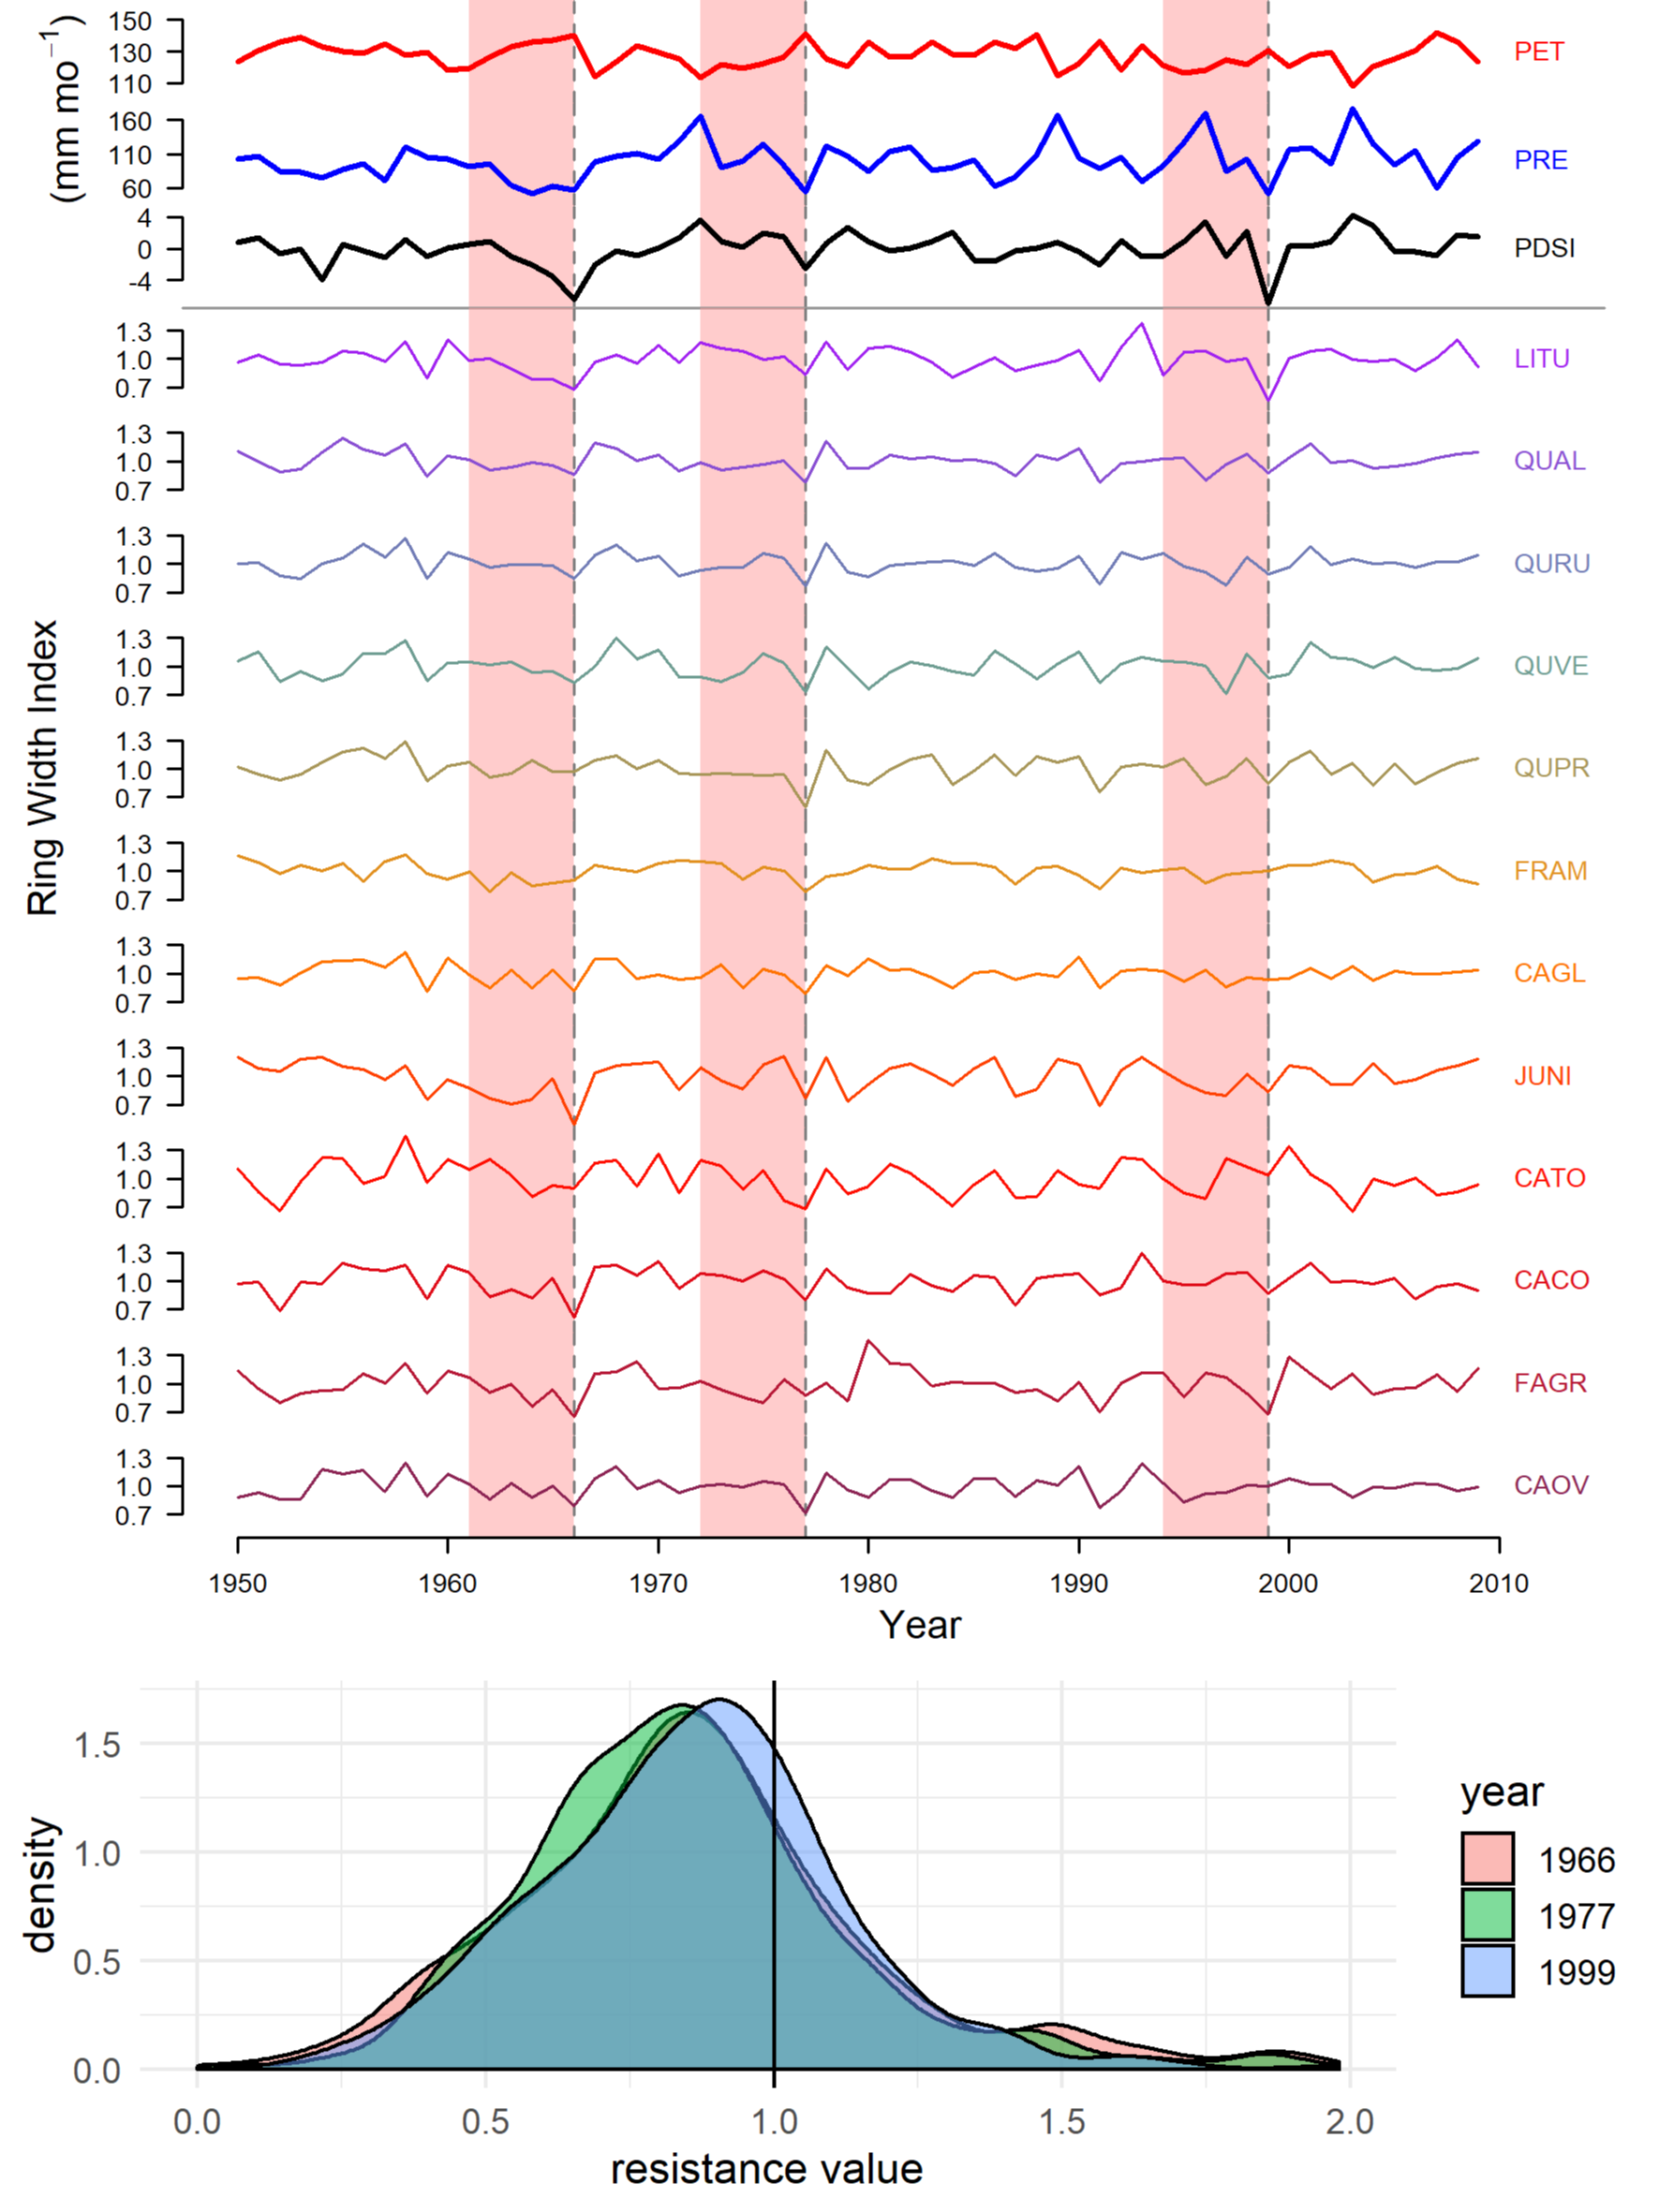
\includegraphics[width=5.20833in,height=\textheight]{tables_figures/Figure1.png}
\caption{\textbf{Figure 1. Climate and species-level growth responses
over our study period, highlighting the three focal drougths (a) and
community-wide responses} Time series plot (a) shows peak growing season
(May-August) climate conditions and residual chronologies for each
species. Focal droughts are indicated by dashed lines, and shading
indicates the pre-drought period used in calculations of the resistance
metric. Figure modified from \citep{helcoski_growing_2019}. Density
plots (b) show community- wide resistance values for each drought.}
\end{figure}

In the 60-year period between 1950 and 2009, there were three droughts
that met our criteria of anomalously dry climatic conditions coupled
with substantial reductions in tree growth for at least some portions of
the community: 1966, 1977, and 1999 (Fig. 1). We excluded one year
(1991) meeting the growth reduction criteria (26.5\% of trees
experienced \textgreater{}30\% growth reduction, mean resistance=
-13.8\%) because this year was not among the strongest droughts of the
study period (\textbf{DETAILS}). Rather, the severity of growth
reduction may be explained by defoliation by gypsy moths
(\emph{Lymantria dispar} L.) from approximately 1988-1995, which most
stronly impacted \emph{Quercus} spp. (\emph{Cite Shenandoah paper, if
accepted}). Climatically, these droughts included three of the five
years between 1950 and 2009 with greatest moisture deficit (PET-PRE)
during the peak growing season months of May-August, which are the
months to which annual tree growth at this site is most sensitive
\citep{helcoski_growing_2019}. Specifically, 1966, 1977, and 1999 had
mean MJJA PET-PRE of 83.37, 86.97, and 80 mm mo-1, respectively. The
years 1964 and 2007 also ranked in the top five driest (PET-PRE =83.87
and 82.13 mm mo-1), but \emph{were not among the lowest in terms of PDSI
and were not identified as a pointer yeasr.} \textbf{The droughts
differed in timing/duration/etc. .. The year 1966 was preceded by two
relatively dry years\ldots{} 1964 among five driest in terms of
May-August {[}PET-PRE{]}, 1965 also anomalously hot and dry. }

Community-level tree growth responses to these droughts were modest,
with modal resistance values of \#, \#, and \# for 1966, 1977, and 1999,
respectively (Fig. 1b). In each drought, roughly 30\% of the cored trees
suffered \(\ge\) 30\% growth reductions (\(R\) \(\le\) 0.7): \#\% in
1966, \#2\% un 1977, and \#\% in 1999. \emph{Some} trees exhibited
increased growth: (\(R\) \textgreater{} 1.0): \#\% in 1966, \#\% in
1977, and \#\% in 1999.

\emph{Tree size and drought resistance}

Overall, our analysis confirmed the tendency for larger-diameter trees
to show greater reductions in growth during drought
\citep{bennett_larger_2015} (\emph{H1.0}), although there was no
signficant effect for 1977 or 1999 individually (Tables 1, 4). The same
held true for \(ln[H]\) as a univariate predictor (\emph{H1.1}; Tables
1, 4). When combined with other predictor variariables in our
multivariate models, the top models usually included an effect of
\(ln[H]\), and its coefficient was consistently negative, as predicted
(Tables 1, 5). We note that a non-signficant positive correlation
between \(ln[H]\) and \(R\) for 1999 became negative in the context of
the multivariate models, again supporting \emph{H1.1} (Table 1).

\begin{table}[!h]

\caption{\label{tab:unnamed-chunk-3}**Table 4. Univariate models**}
\centering
\resizebox{\linewidth}{!}{
\fontsize{12}{14}\selectfont
\begin{tabular}{llllrllllll}
\toprule
\multicolumn{1}{c}{ } & \multicolumn{1}{c}{ } & \multicolumn{1}{c}{ } & \multicolumn{2}{c}{all droughts} & \multicolumn{2}{c}{1966} & \multicolumn{2}{c}{1977} & \multicolumn{2}{c}{1999} \\
\cmidrule(l{3pt}r{3pt}){4-5} \cmidrule(l{3pt}r{3pt}){6-7} \cmidrule(l{3pt}r{3pt}){8-9} \cmidrule(l{3pt}r{3pt}){10-11}
variable & category & null variables & dAICc & coefficients & dAICc & coefficients & dAICc & coefficients & dAICc & coefficients\\
\midrule
drought year & 1966 &  & -2.42 & 0.0000 & - & - & - & - & - & -\\
 & 1977 &  & - & -0.0209 & - & - & - & - & - & -\\
 & 1999 &  & - & -0.0105 & - & - & - & - & - & -\\
ln[DBH] &  & Y & 8.17 & -0.0385 & 15.32 & -0.0888 & -0.87 & -0.0214 & -1.93 & 0.0057\\
ln[height] &  & Y & 8.8 & -0.0648 & 15.27 & -0.1443 & -0.98 & -0.0335 & -2.03 & 0.0018\\
\addlinespace
crown position & D & Y & -2.96 & -0.0461 & 3.25 & -0.0509 & 0.66 & -0.0759 & 0.38 & -0.0103\\
(alone) & C &  & - & 0.0000 & - & 0 & - & 0 & - & 0\\
 & I &  & - & -0.0063 & - & 0.0732 & - & -0.0298 & - & -0.0563\\
 & S &  & - & 0.0122 & - & 0.0526 & - & 0.0432 & - & -0.0483\\
crown position & D & ln[H]+Y & 0.55 & -0.0364 & -1.41 & -0.0359 & -0.24 & -0.074 & 3.99 & -0.0027\\
\addlinespace
(with height) & C &  & - & 0.0000 & - & 0 & - & 0 & - & 0\\
 & I &  & - & -0.0406 & - & 0.0177 & - & -0.0363 & - & -0.0823\\
 & S &  & - & -0.0586 & - & -0.0654 & - & 0.03 & - & -0.1011\\
ln[TWI] &  & ln[H]+Y & 5.33 & -0.0886 & -1.96 & -0.0168 & 5.06 & -0.1406 & 2.72 & -0.1025\\
ln[TWI]*ln[H] &  & ln[H]+ln[T]+Y & -1.18 & 0.0677 & -1.75 & 0.0749 & -1.86 & 0.0533 & -1.79 & 0.0566\\
\addlinespace
wood density &  & ln[H]+Y & -1.89 & -0.0498 & -1.1 & -0.2161 & -1.19 & -0.1827 & 0.23 & 0.2512\\
leaf mass per area &  & ln[H]+Y & -2 & 0.0003 & -1.89 & 0.0011 & -1.74 & -0.0014 & -1.99 & 0.0005\\
ring porosity & ring & ln[H]+Y & -2.4 & 0.0574 & 1.78 & 0.151 & 0.59 & -0.1879 & 4.25 & 0.2025\\
 & semi-ring &  & - & -0.0335 & - & -0.1324 & - & -0.1426 & - & 0.1516\\
 & diffuse &  & - & 0.0000 & - & 0 & - & 0 & - & 0\\
\addlinespace
turgor loss point &  & ln[H]+Y & 1.22 & -0.1675 & -1.78 & -0.0845 & 1.14 & -0.2432 & 0.06 & -0.1749\\
percent loss area &  & ln[H]+Y & 7.89 & -0.0138 & 9.82 & -0.0244 & -0.07 & -0.0104 & -0.73 & -0.0074\\
\bottomrule
\end{tabular}}
\end{table}

\begin{table}[!h]

\caption{\label{tab:unnamed-chunk-4}**Table 5. Summary of R\^2 and coefficients of the best multivariate models for each drought instance.** Models are ranked by AIC, and we show all models whose AIC value falls within 2.0 of the best model (dAICc<2).}
\centering
\resizebox{\linewidth}{!}{
\fontsize{12}{14}\selectfont
\begin{tabular}{lrrrlllllllllll}
\toprule
\multicolumn{1}{c}{ } & \multicolumn{1}{c}{ } & \multicolumn{1}{c}{ } & \multicolumn{1}{c}{ } & \multicolumn{1}{c}{ } & \multicolumn{4}{c}{crown position} & \multicolumn{1}{c}{ } & \multicolumn{3}{c}{xylem architecture} & \multicolumn{1}{c}{ } & \multicolumn{1}{c}{ } \\
\cmidrule(l{3pt}r{3pt}){6-9} \cmidrule(l{3pt}r{3pt}){11-13}
drought & dAICc & R2 & Intercept & ln[H] & D & C & I & S & ln[TWI] & diffuse & semi-ring & ring & PLA & TLP\\
\midrule
\addlinespace[.4em]
\multicolumn{1}{l}{\textbf{}}\\
\hspace{1em}all & 0.000 & 0.11 & 1.108 & -0.062 & - & - & - & - & -0.085 & - & - & - & -0.012 & -0.105\\
\hspace{1em} & 0.338 & 0.10 & 1.494 & -0.097 & -0.036 & 0 & -0.038 & -0.056 & -0.078 & - & - & - & -0.013 & -\\
\hspace{1em} & 0.403 & 0.12 & 1.263 & -0.096 & -0.035 & 0 & -0.036 & -0.053 & -0.078 & - & - & - & -0.012 & -0.087\\
\hspace{1em} & 0.515 & 0.12 & 1.393 & -0.064 & - & - & - & - & -0.087 & 0 & 0.147 & 0.048 & -0.017 & -\\
\hspace{1em} & 0.571 & 0.10 & 1.375 & -0.061 & - & - & - & - & -0.085 & - & - & - & -0.013 & -\\
\hspace{1em} & 0.903 & 0.12 & 1.492 & -0.098 & -0.034 & 0 & -0.036 & -0.053 & -0.079 & 0 & 0.122 & 0.049 & -0.016 & -\\
\addlinespace[.4em]
\hline
\multicolumn{1}{l}{\textbf{}}\\
\hspace{1em}1996 & 0.000 & 0.26 & 2.271 & -0.153 & - & - & - & - & - & 0 & 0.35 & 0.152 & -0.035 & 0.25\\
\hspace{1em} & 0.537 & 0.26 & 1.537 & -0.154 & - & - & - & - & - & 0 & 0.098 & 0.133 & -0.023 & -\\
\hspace{1em} & 1.093 & 0.27 & 2.389 & -0.177 & -0.038 & 0 & 0.016 & -0.068 & - & 0 & 0.352 & 0.153 & -0.035 & 0.27\\
\hspace{1em} & 1.434 & 0.24 & 1.629 & -0.143 & - & - & - & - & - & - & - & - & -0.024 & -\\
\hspace{1em} & 1.982 & 0.26 & 2.307 & -0.152 & - & - & - & - & -0.016 & 0 & 0.356 & 0.152 & -0.035 & 0.254\\
\addlinespace[.4em]
\hline
\multicolumn{1}{l}{\textbf{}}\\
\hspace{1em}1977 & 0.000 & 0.22 & 0.346 & - & -0.074 & 0 & -0.027 & 0.042 & -0.131 & 0 & -0.331 & -0.23 & - & -0.384\\
\hspace{1em} & 0.090 & 0.21 & 0.393 & - & - & - & - & - & -0.14 & 0 & -0.324 & -0.234 & - & -0.369\\
\hspace{1em} & 1.116 & 0.21 & 0.460 & -0.026 & - & - & - & - & -0.137 & 0 & -0.316 & -0.225 & - & -0.367\\
\hspace{1em} & 1.914 & 0.22 & 0.367 & -0.006 & -0.073 & 0 & -0.029 & 0.037 & -0.13 & 0 & -0.33 & -0.229 & - & -0.383\\
\addlinespace[.4em]
\hline
\multicolumn{1}{l}{\textbf{}}\\
\hspace{1em}1999 & 0.000 & 0.25 & 1.284 & -0.081 & 0.003 & 0 & -0.077 & -0.095 & -0.087 & 0 & 0.22 & 0.193 & -0.008 & -\\
\hspace{1em} & 0.085 & 0.25 & 0.844 & -0.082 & 0.001 & 0 & -0.078 & -0.095 & -0.085 & 0 & 0.062 & 0.185 & - & -0.142\\
\hspace{1em} & 0.462 & 0.23 & 1.174 & -0.083 & 0.002 & 0 & -0.079 & -0.099 & -0.088 & 0 & 0.135 & 0.2 & - & -\\
\hspace{1em} & 0.956 & 0.24 & 1.042 & - & - & - & - & - & -0.1 & 0 & 0.261 & 0.191 & -0.01 & -\\
\hspace{1em} & 1.029 & 0.24 & 0.700 & -0.09 & -0.002 & 0 & -0.082 & -0.101 & - & 0 & 0.046 & 0.185 & - & -0.151\\
\hspace{1em} & 1.193 & 0.24 & 1.159 & -0.089 & 0 & 0 & -0.081 & -0.101 & - & 0 & 0.21 & 0.194 & -0.008 & -\\
\hspace{1em} & 1.326 & 0.24 & 0.533 & - & - & - & - & - & -0.098 & 0 & 0.077 & 0.181 & - & -0.161\\
\hspace{1em} & 1.849 & 0.26 & 1.046 & -0.079 & 0.002 & 0 & -0.077 & -0.094 & -0.086 & 0 & 0.14 & 0.188 & -0.005 & -0.078\\
\hspace{1em} & 1.851 & 0.22 & 1.045 & -0.092 & -0.001 & 0 & -0.084 & -0.105 & - & 0 & 0.123 & 0.201 & - & -\\
\bottomrule
\end{tabular}}
\end{table}

Crown position was generally correlated with \(H\), but with substantial
variation (Fig. 2\textbf{e}). Crown position was a much poorer predictor
of \(R\) than was \(H\) (Table 4), lending little overall support to
\emph{H1.2} (Table 1). When considered alone, \(CP\) had a significant
influence only in the 1977 drought, during which trees with dominant
\(CP\) had the lowest \(R\). When considered in conjunction with \(H\),
\(CP\) came out as a significant predictor only for the 1999 drought,
during which suppressed trees had the lowest \(R\). Crown position was
included in \textbf{roughly half} of the top models, with mixed results
as to how \(R\) varied with \(CP\) (Table 5). Most commonly in these
multivariate models, as in the univariate models (Table 4), the
resistance of dominant trees was less than that of co-dominant trees but
higher that of suppressed trees. Thus, \(CP\) was sometimes a useful
predictor of \(R\), but overall had a weak effect relative to that of
\(H\).

In the non-drought years for which we have vertical profiles in climate
data (\textbf{YEARS}), taller trees--or those in dominant crown
positions-- were generally exposed to higher evaporative demand during
the peak growing season months (May-August; Fig. 2). Specifically,
maximum daily wind speeds were signficantly higher above the top of the
canopy (40-50m) than within and below (10-30m) (Fig. 2a). Relative
humidity was also somewhat lower during June-August, ranging from
\textasciitilde{}50-80 above the canopy and \textasciitilde{}60-90\% in
the understory (Fig. 2b). Air temperature did not vary across the
vertical profile (Fig. 2c). {[}\textbf{biological temperature?- probably
drop}{]}

\begin{figure}
\centering
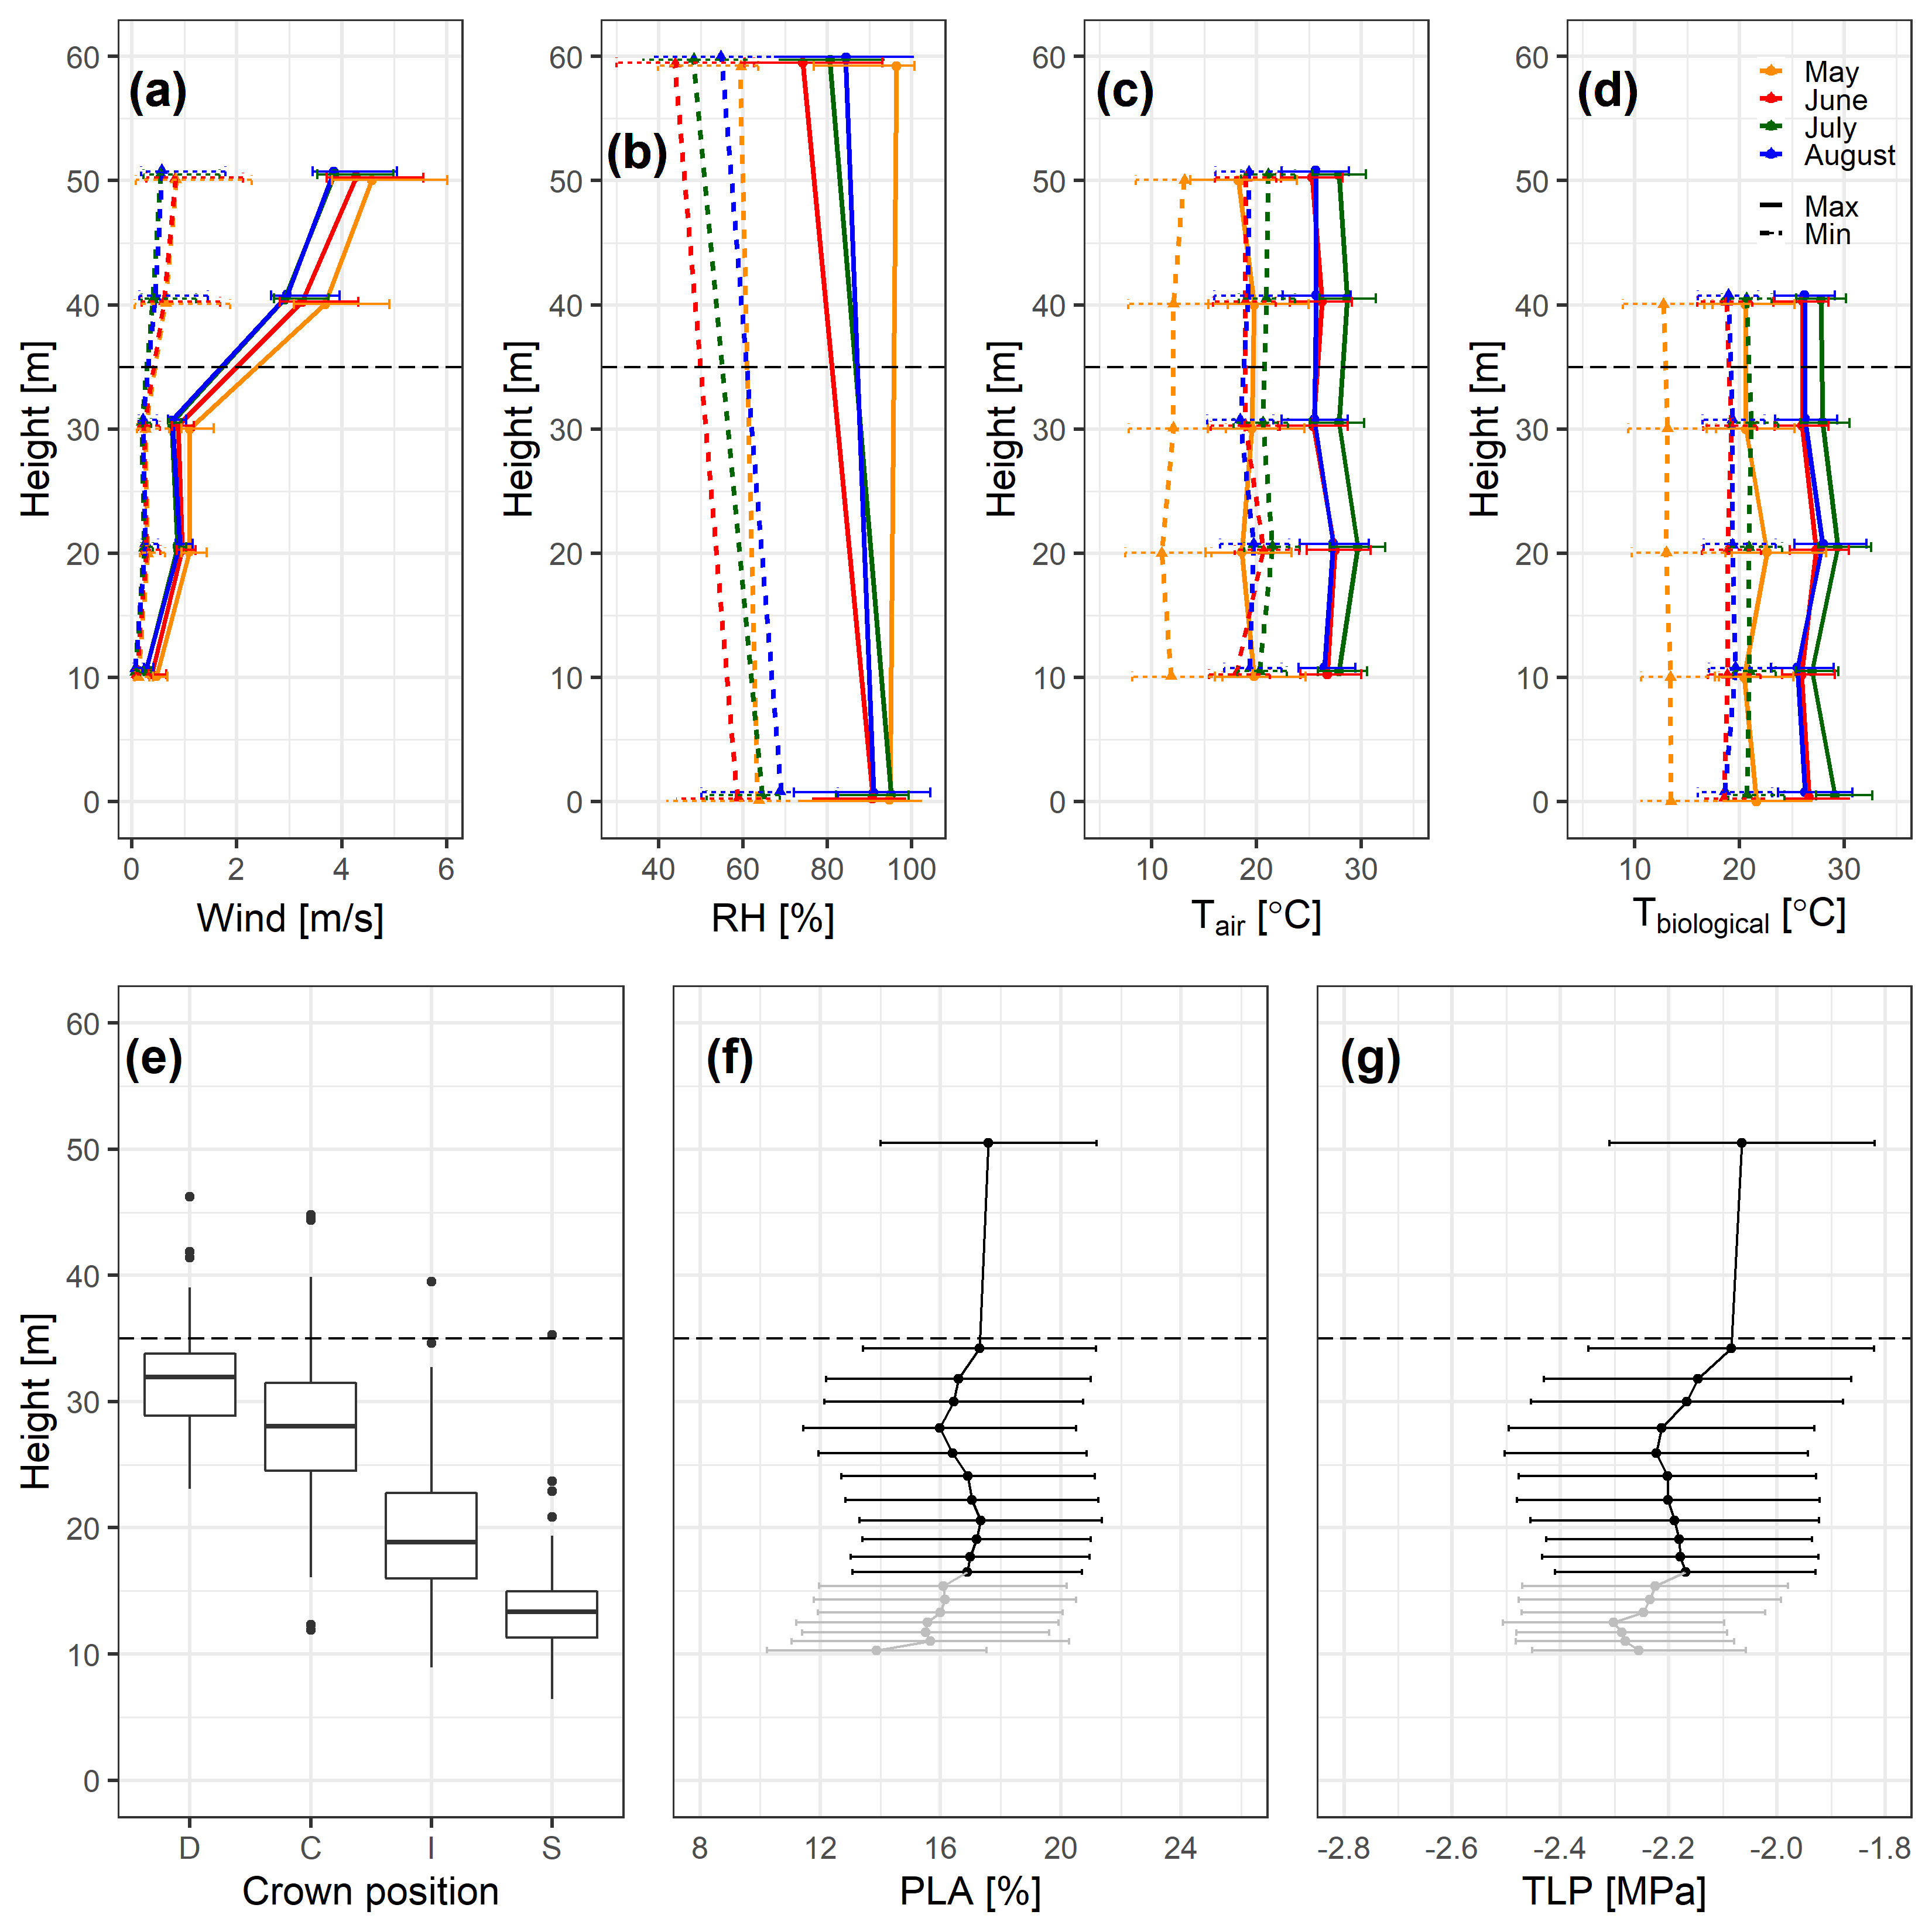
\includegraphics[width=5.20833in,height=\textheight]{tables_figures/Figure2.png}
\caption{\textbf{Figure 2. Height profiles in growing season climatic
conditions, tree heights by crown position, and leaf hydraulic traits}
The top row shows averages (\(\pm\) SD) of daily maxima and minima of
(a) wind speed, (b) relative humidity (\(RH\)), (c) air temperature
(\(T_{air}\)), and (d) biological temperature
(\(T_{biological}\))averaged over each month of the peak growing season
(May-August) from YEAR-YEAR. In these plots, heights are slightly offset
for visualization purposes. Also shown are (e) 2018 tree heights by
canopy position (see Table 2 for codes) and vertical profiles in (f)
\(PLA_{dry}\) and (g) \(\pi_{tlp}\). In (f-g), values are community-wide
averages across height bins (plotted at upper end of height bin), with
grey indicating bins for which species-level trait measurements are
available for \textless{}75\% of individuals. In all plots, the dahsed
horizontal line indicates the 95th percentile of tree heigts in the
ForestGEO plot.}
\end{figure}

Resistance was negatively correlated with \(ln[TWI]\) (Tables 4-5),
negating the idea that trees in moist microsites would suffer less
during drought. Nevertheless, we tested for a negative
\(ln[H] *ln[TWI]\) interaction (\emph{H1.3}), which could indicate that
smaller trees (with smaller rooting volume) have a greater tendency to
suffer more in drier microenvironments with greater depth to the water
table. \emph{H1.3} was rejected; the \(ln[H] *ln[TWI]\) interaction was
never signficant and had a consistently positive coefficient (Table 4).

\emph{Species' traits, height, and drought resistance}

We partially support \emph{H2.1}: Species' hydraulic traits --\(XP\),
\(PLA_{dry}\), and \(\pi_{tlp}\)--were useful in explaining variation in
drought responses, whereas \(LMA\) and \(WD\) were not (Tables 1,4,5).
Specifically, \(LMA\) and \(WD\) never significantly associated with
\(R\) in the univariate models (all dAIC \(\le\) 0.23; Table 4), and
therefore these were excluded as candidate variables for the full
multivariate models. In contrast, \(XP\), \(PLA_{dry}\), and
\(\pi_{tlp}\) all explained at least modest amounts of variation (dAIC
\textgreater{} 1.0) in at least one drought (Table 4). Of these,
\(PLA_{dry}\) was the strongest predictor, with consistently negative
coefficients across all droughts. \(\pi_{tlp}\) never came out as
significant (dAIC \(\ge\) 2) in the univariate models, but had a
consistently negative coefficient (Table 4). Whereas ring-porous species
had highest \(R\) overall and in the 1966 and 1999 droughts, they had
lower \(R\) in 1977. Results were similar in the context of multivariate
models (Table 5), except that \(\pi_{tlp}\) had a positive coefficient
in the 1966 models in which it was included.

We reject \emph{H2.2}, finding no evidence that taller trees tend to
have traits associated with greater drought resistance. In part because
of the large sample size (n=\# trees--all individuals of our 12 focal
species \(\ge\) 10 cm in 25.6 ha \textbf{Ian, confirm}), there were very
significant (p\textless{}0.0001) correlations of \(H\) with all species'
traits (\textbf{SI Table?}). However, the correlation only matched the
predicted direction (\emph{i.e.}, more drought-resistant traits
associated to taller trees) in the case of \(LMA\), which did not
correlate with \(R\). Furthermore, although correlations were
statistically signifcant, trait variation within each height class
overwhelmed any vertical trends (Fig. 2\textbf{f-g}).

We support the hypothesis (\emph{H2.3}) that the observed tendency for
larger trees to have greater growth reductions during drought (lower
\(R\)) is \emph{not} driven by more drought-sensitive traits in larger
trees, but rather by size itself (Tables 1,5). As discussed above, there
was little meaningful variation in traits with height at the community
level. When \(ln[H]\) and hydraulic traits were considered together in
multivariate models, the effect of \(ln[H]\) on \(R\) was consistently
negative (Table 5)--reversing a non-signficant positive \(ln[H]\)-\(R\)
correlation in the univariate model for the 1999 drought (Table 4).

\emph{Responses across droughts}

We reject the hypothesis (\emph{H3.1}) that overall community responses
varied across droughts. Within the context of mixed effects models,
there were no significant differences in \(R\) across drought years
(Table 4). This is consistent with the observation that the distribution
of \(R\) values was similar across droughts (Fig. 1b).

We mostly reject the hyopthesis (\emph{H3.2}) that directions of
responses varied across droughts. In the majority of cases, response
directions were consistent across droughts in both univariate and
multivariate models (Tables 1,4,5). However, there were a few
exceptions--most commonly in the categorical variables (\(CP\) and
\(XP\)) but also for \(\pi_{tlp}\) in the multivariate model for the
1966 drought; Tables 4, 5). These differences may very well be random,
as opposed to statistically meaningful. Among the univariate models,
there was no instance predictor variables signficantly improved the
models of two different droughts (dAIC \(\ge\) 2), but with contrasting
coefficients (Table 4). Among the multivariate models, \(CP\) was not
consistently in the top models for any drought (Table 5), and
\(\pi_{tlp}\) only appeared with a positive coefficient in two of five
models for the 1966 drought (contrasting with a negative coefficient in
the univariate model; Table 4). The difference most likely to be real is
that ring and semi-ring porous species had lower resistance than diffuse
porous species in the 1977 drought, contrasting with higher resistance
in 1966 and 1999 (Tables 4,5), but note that \(XP\) was not a signficant
predictor on its own for the 1977 drought.

We support the hypothesis (\emph{H3.3}) that the strength of predictor
variables was different across the droughts (Tables 1,4,5). For
instance, \(ln[H]\) and \(PLA_{dry}\) had much stronger negative effects
in 1966 than in the other two years, \(ln[TWI]\) had the strongest
negative effect in 1977, and \(CP\) (lowest \(R\) among supressed trees)
and \(XP\) (lowest \(R\) among diffuse-porous trees) were strongest in
1999 (Tables 4,5).

\hypertarget{discussion}{%
\subsubsection{Discussion}\label{discussion}}

Our results reveal how tree size, microhabitat, and hydraulic traits
shaped tree growth responses across three droughts in a temperate
deciduous forest (Table 1). The tendencey for larger trees to suffer
more, observed here as in forests around the world (\textbf{REFS}), was
driven primarily by their height. There was a marginal additional effect
of crown exposure, with the most exposed and the most suppressed trees
suffering most--consistent with observations of both greater drought
sensitivity of exposed trees (e.g., \citep{suarez_factors_2004};
\citep{scharnweber_confessions_2019}; MORE??) and greater sensitivity of
suppressed and crowded individuals (\textbf{REFS- }). There was no
evidence that root water access increased drougth resistance; in
contrast, trees in wetter topographic positions suffered more
(consistent with
\href{https://repository.si.edu/bitstream/handle/10088/32814/Zuleta-et-al_2017_Ecology.pdf?sequence=1\&isAllowed=y}{Zuleta
et al.}), and larger rooting volume provided no advantage in the drier
microenvironments. The lower drought resistance of larger trees was not
driven by any tendency for the canopy to be dominated by more
drought-sensitive species. Drought-sensitive species were not linked to
\(LMA\) and \(WD\) but were predicted by hydraulic traits
(\(PLA_{dry}\), \(\pi_{tlp}\), and \(XP\)), which is physiologically
logical (\textbf{REFS}\citep{kannenberg_linking_2019}) but
scientifically novel in that \(PLA_{dry}\) and \(\pi_{tlp}\) have not
previously been linked to drought growth responses. The direction of
these responses was mostly consistent across droughts, indicating that
they were driven by fundamental physiological mechanisms; however, the
strengths of each predictor varied across droughts, indicating that
specific drought characteristics interact with tree size,
microenvironment, and traits to shape which individuals suffer most.
These findings significantly advance our knowledge as to the factors
that confer vulnerability or resilience on trees during drought.

The droughts considered here were of similar severity (Fig. 1b) and
fairly moderate; droughts of this magnitude have occurred with an
average frequency of approximately one per 10-15 years (Fig. 1a,
\citet{helcoski_growing_2019}). Therefore, we excpect that most species
are adapted, and individual trees acclimatized, to survive droughts of
this nature. While the majority of trees experienced reduced growth, a
substantial portion had increased growth (Fig. 1b), underlining the fact
that these droughts did not induce extreme stress on the entire forest.
It is likely for this reason, combined with the fact that many factors
other than climate affect tree growth in closed-canopy forests, that our
best models characterize only a modest amount of variation: 10-12\% for
all droughts combined, and 21-27\% for each individual drought (Table
5). Methodologically, the moderate nature of these drougths is an
advantage because our analysis considers only trees that survived all of
these droughts, and we lack information on the trees that were killed.
These are likely to be relatively modest in number, and local forest
monitoring data stretching back to the late 1980s confirms that the 1999
drought did not trigger major declines in tree abundance or biomass
(\emph{Anderson-Teixeira et al., in review}). Thus, the droughts
considered here are substantially weaker than those that have triggered
massive tree die-off (e.g.,
\href{https://doi.org/10.1016/j.foreco.2009.09.001}{Allen et al.~2015}),
many of which have shaped our understanding about the role of tree size
(Bennett et al.~2015; Stovall et al.~2019) and--to some extent-- traits
(\textbf{REFS}). Nevertheless, our results are consistent with findings
from more extreme droughts.

Our analysis indicates that height is the primary factor through which
tree size mediates drought response; however, specific identification of
the primary physiological mechanism(s) is complicated by the fact that
multiple drought-relevant environmental parameters and tree
characteristics covary with height. To begin with, taller trees face
inherent biophysical challenges in lifting water a greater distance
against the effects of gravity and friction (\textbf{REFS}). They also
face different microenvironments, which are partially related to canopy
position. Even under non-drought conditions, evaporative demand
increases with tree height, which are more closely coupled to the
atmosphere (Fig. 1a-b; \textbf{REFS- Jarvis 1984?};
\href{https://nph-onlinelibrary-wiley-com.smithsonian.idm.oclc.org/doi/full/10.1111/nph.15071}{Bretfeld
et al}). \textbf{The vegetation reaches higher
temperatures\href{https://github.com/SCBI-ForestGEO/McGregor_climate-sensitivity-variation/issues/58}{??}},
which would occur more during a drought when solar radiation tends to be
higher and less water is available for evaporative cooling of the
leaves. Furthermore, daytime CO\_2 concentrations tend to be lower in
the canopy than in the understory \textbf{(Fig.
2\href{https://github.com/SCBI-ForestGEO/McGregor_climate-sensitivity-variation/issues/58}{??}}
(\href{https://watermark.silverchair.com/21-12-13-951.pdf}{Koike et
al.~2001}; MORE REFS), implying greater water costs of \(CO_2\) uptake.
\textbf{{[}McDowell-vertical profiles in isotopes?*{]}}. Taller trees
are more likely to be in domiant canopy positions, although signficant
decoupling can be introduced by the configuration of neighboring trees
(Fig. 2\textbf{e?})
(\href{https://www.ncbi.nlm.nih.gov/pubmed/16643303}{Mueller-Landau et
al.~2016}). We show that height is a far stronger predictor than crown
position (Tables 1,4,5). Our analysis does have the limitation that
canopy positions were recored in 2018 and undoubtedly changed for some
trees since the 1960s, and we note that \(CP\) became an increasingly
poor predictor moving from 1999 back to 1966 (Table 4). However, rates
of change are relatively slow, and the fact that some trees inevitably
did grow towards more dominant positions would bias against the
acceptance of (\emph{H1.2}), implying that dominant crown positions did
indeed reduce \(R\), which makes sense in light of the vertical
enviromnental gradients described above and agrees with previous studies
showing greater drought sensitivity in more exposed trees
(\citep{suarez_factors_2004}; \citep{scharnweber_confessions_2019};
MORE??). It is safe to assume that currently suppressed trees have
always been suppressed, and their relatively low \(R\) (after correcting
for height effects) is real, which is consistent with analyses showing
that suppressed--and particularly crowded--trees can suffer
distproportionately during drought (\textbf{REFS}). The observed
height-sensitivity of \(R\), together with the apparent lack of
importance of root water access (\emph{H1.3}), agrees with the concept
that physiological limitations to transpiration under drought shift from
root water access to the plant-atmosphere intreface as forests age
(\href{https://nph-onlinelibrary-wiley-com.smithsonian.idm.oclc.org/doi/full/10.1111/nph.15071}{Bretfeld
et al}), such that tall trees--particularly the very tallest--are the
most sensitive in mature forests. Additional research comparing drought
responses of young and old forest stands, along with and short and tall
isolated trees, would be valuable for more clearly disentanging the
roles of tree height and crown exposure.

Beyond microenvironment, multiple tree characteristics covary with
height. To begin with, multiple tree characteristics that may influence
drought resistance scale with \(DBH\)--or, similarly, \(H\)--including
crown volume, rooting volume, sapwood area, transpiration \ldots{}
(e.g.,
\href{https://besjournals.onlinelibrary.wiley.com/doi/abs/10.1111/1365-2435.12470}{Anderson-Teixeira
et al.~2015\_scaling}; \textbf{REFS--KAT: Sperry scaling model; roots
reference; BAAD database?}). These work in combination to shape
whole-plant hydraulic function (\textbf{REFS-KAT: Sperry scaling model,
check McDowell scaling paper, Couvreur et al.~2018; others?}), and we
cannot expect to statistically identify a single driver that fully
encapsulates size-related variation in trees. However, height is
arguably the most biophysically meaningful tree-size variable shaping
drought response. Beyond whole-plant characteristics, leaf traits vary
with height on the tree--sometimes quite dramatically, with upper-canopy
leaves \ldots{} (\textbf{describe differences})
(\href{https://onlinelibrary-wiley-com.smithsonian.idm.oclc.org/doi/full/10.1111/pce.13322?casa_token=92wZmmL9EhQAAAAA\%3A2cq5yAR0_pyM9TVBa5o_DKkhDuHwIUFryxZ43zsdTgQyEa8f0ZfiEHZ5SHV7fFB49UkzXNvL7nMwabU}{Couvreur
et al.~2018};
\href{https://watermark.silverchair.com/21-12-13-951.pdf}{Koike et
al.~2001}). Our analysis focuses on species-level comparisons and does
not characterize the role of variation with height. On an individual
level, average leaf characteristics of an individual tree would scale
with its crown height, with taller individuals having on average more
drought-resistant traits--assuming trends for \(PLA_{dry}\) and
\(\pi_{tlp}\), which have not been characterized (\emph{\textbf{LAWREN,
IS THIS TRUE?}), follow the general pattern of increasing drought
resistance with height. In not accounting for this, our analysis is most
likely biased in a conservative direction when assessing }H2.3* (Table
1)--\emph{i.e.}, accounting traits on an individual level should result
in a stronger negative effect of \(ln[H]\). Further characterization of
leaf hydraulic traits in relation to height and crown exposure would be
valuable for enhancing our understanding of the interactive effects of
tree height and traits on drought responses (\emph{Couvreur et
al.~2018}).

The development of tree-ring chronologies for all dominant tree species
at our site \citep{helcoski_growing_2019} made it possible to compare
historical drought responses across 12 species and their associated
traits at a single site for the first time (\textbf{verify- Neil,
Alan}). Concerted measurement of leaf hydraulic traits of emerging
importance (\textbf{REFS--KAT/NOBBY/LAWREN}) allowed novel insights into
the role of hydraulic traits in shaping drought response. The finding
that \(PLA_{dry}\) and \(\pi_{tlp}\) are useful for predicting drought
responses is consistent with studies demonstrating that these are
physiolgoically meaningful traits linked to species distribution along
moisture gradients (\textbf{REFS--KAT/NOBBY/LAWREN}),
\textbf{MORE--KAT/NOBBY/LAWREN}\ldots{} (\textbf{REFS}). It is
scientifically exciting in that it indicates that these traits, which
can be measured relatively easily \(PLA_{dry}\) and \(\pi_{tlp}\)
(\textbf{REFS--KAT/NOBBY/LAWREN}), hold promise for predicting drought
growth responses across species. The importance of linking species'
traits to drought responses increases with tree species diversity;
whereas it is feasible to study drought responses for all dominant
species in most boreal and temperate forests (e.g., this study;
\textbf{REFS}), this becomes difficult to impossible for diverse
tropical forests, where linking hydraulic traits to drought responses
would be invaluable for forecasting how little-known species and whole
forests will respond to future droughts
(\textbf{REFS--KAT/NOBBY/LAWREN}).

Although the physiological mechanisms discussed above lead to generally
consistent directions of growth responses to tree height and hydaulic
traits across droughts, indicating the universality of the underlying
mechanisms, the relative importantance of the drivers varied widely
across droughts, indicating an interaction with drought characteristics
(Tables 4-5). {[}\textbf{BRIEFLY DISCUSS DIFFERENCES ACROSS DROUGHTS--
For example, 1966 was preceded by two dry years, and height had the
strongest effect in this drought, consistent with the finding that
height becomes a stronger predictor of mortality as drought duration and
intensity increase (Stovall et al.~2019). \ldots{}}{]} Of course, site
characteristics also define the nature of droughts, and comparisons of
size and trait effects across sites would be of great value to
elucidating the mechanisms through which these shape drought resistance
(\textbf{check for refs}). Unfortunately, our ability to compare forest
responses across droughts is hampered by the fact that droughts are
rarely explicitly defined in ecological studies \citep{slette_how_2019}.
Further research will be required to understand how drought
characteristics interact with driver variables to shape tree growth
responses.

As climate change drives increasing drought in many of the world's
forests (\emph{REFS-KAT}), the fate of forests and their climate
feedbacks will be shaped by the biophysical and physiological drivers
observed here. Large trees have been suffering disrpoportionately in
forests around the world (\emph{REFS}), and we here show that this is
primarily driven by their height, with some contributions from canopy
position. The distinction is important because it suggests that height
\emph{per se} makes trees vulnerable, even if their crowns are somewhat
protected by neighbors, whereas solitary trees or the dominant trees in
young regrowth forests should be less vulnerable. Considering just
height and crown position, this would suggest that mature forests would
be more vulnerable to drought than young forests with short trees;
however, root water access may limit the young forests (Bretfield et
al.), and species traits often shift as forests age, with early
successional species tending to have lower wood densities and higher
hydraulic conductivities that facilitate rapid growth (\textbf{REFS in
Bretfield-beginning of discussion}). The later successional species at
our site (\emph{Fagus grandifolia}, \ldots{} ) have a mix of traits
conferring drought tolerance and resistance (Table 3), and further
research on how hydraulic traits and drought vulnerability change over
the course of succession would be valuable for getting at the very
signficant question of whether old-growth forests are more vulnerable to
drought, and to which types of drought. In the meantime, the results of
this study advance our knowledge of the factors conferring drought
vulnerability and resistance in a mature forest, opening the door for
more accurate forecasting of forest responses to future drought.

\hypertarget{acknowledgements}{%
\subsubsection{Acknowledgements}\label{acknowledgements}}

funding: ForestGEO,

\hypertarget{author-contribution}{%
\subsubsection{Author Contribution}\label{author-contribution}}

words

\newpage

\hypertarget{supplementary-information}{%
\subsubsection{Supplementary
Information}\label{supplementary-information}}

\begin{table}[!h]

\caption{\label{tab:Table S1}Species-specific height regression equations}
\centering
\begin{tabular}{llr}
\toprule
Species & Equations & r.2\\
\midrule
Carya cordiformis & 0.348+0.808*x & 0.879\\
Carya glabra & 0.681+0.704*x & 0.855\\
Carya ovalis & 0.621+0.722*x & 0.916\\
Carya tomentosa & 0.776+0.701*x & 0.894\\
Fagus grandifolia & 0.708+0.662*x & 0.857\\
\addlinespace
Liriodendron tulipifera & 1.32+0.524*x & 0.761\\
Quercus alba & 1.14+0.548*x & 0.647\\
Quercus prinus & 0.44+0.751*x & 0.869\\
Quercus rubra & 1.17+0.533*x & 0.773\\
all & 0.879+0.634*x & 0.857\\
\bottomrule
\end{tabular}
\end{table}

\begin{table}[!h]

\caption{\label{tab:Table S2}Candidate variables for best model}
\centering
\begin{tabular}{rlll}
\toprule
prediction & variable & variable\_description & top\_model\\
\midrule
1.2 & position\_all & crown.position w/height & 1999\\
2.2 & height.ln.m & ln[height] & all\\
2.2 & height.ln.m & ln[height] & 1966\\
2.3 & position\_all & crown.position alone & 1966\\
2.4 & TWI.ln & ln[topographic.wetness.index] & all\\
\addlinespace
2.4 & TWI.ln & ln[topographic.wetness.index] & 1977\\
2.4 & TWI.ln & ln[topographic.wetness.index] & 1999\\
3.1 & rp & ring.porosity & 1966\\
3.1 & rp & ring.porosity & 1999\\
3.2 & PLA\_dry\_percent & percent.loss.area & all\\
\addlinespace
3.2 & PLA\_dry\_percent & percent.loss.area & 1966\\
3.4 & mean\_TLP\_Mpa & mean.turgor.loss.point & all\\
3.4 & mean\_TLP\_Mpa & mean.turgor.loss.point & 1977\\
\bottomrule
\end{tabular}
\end{table}

\begin{figure}[ht]
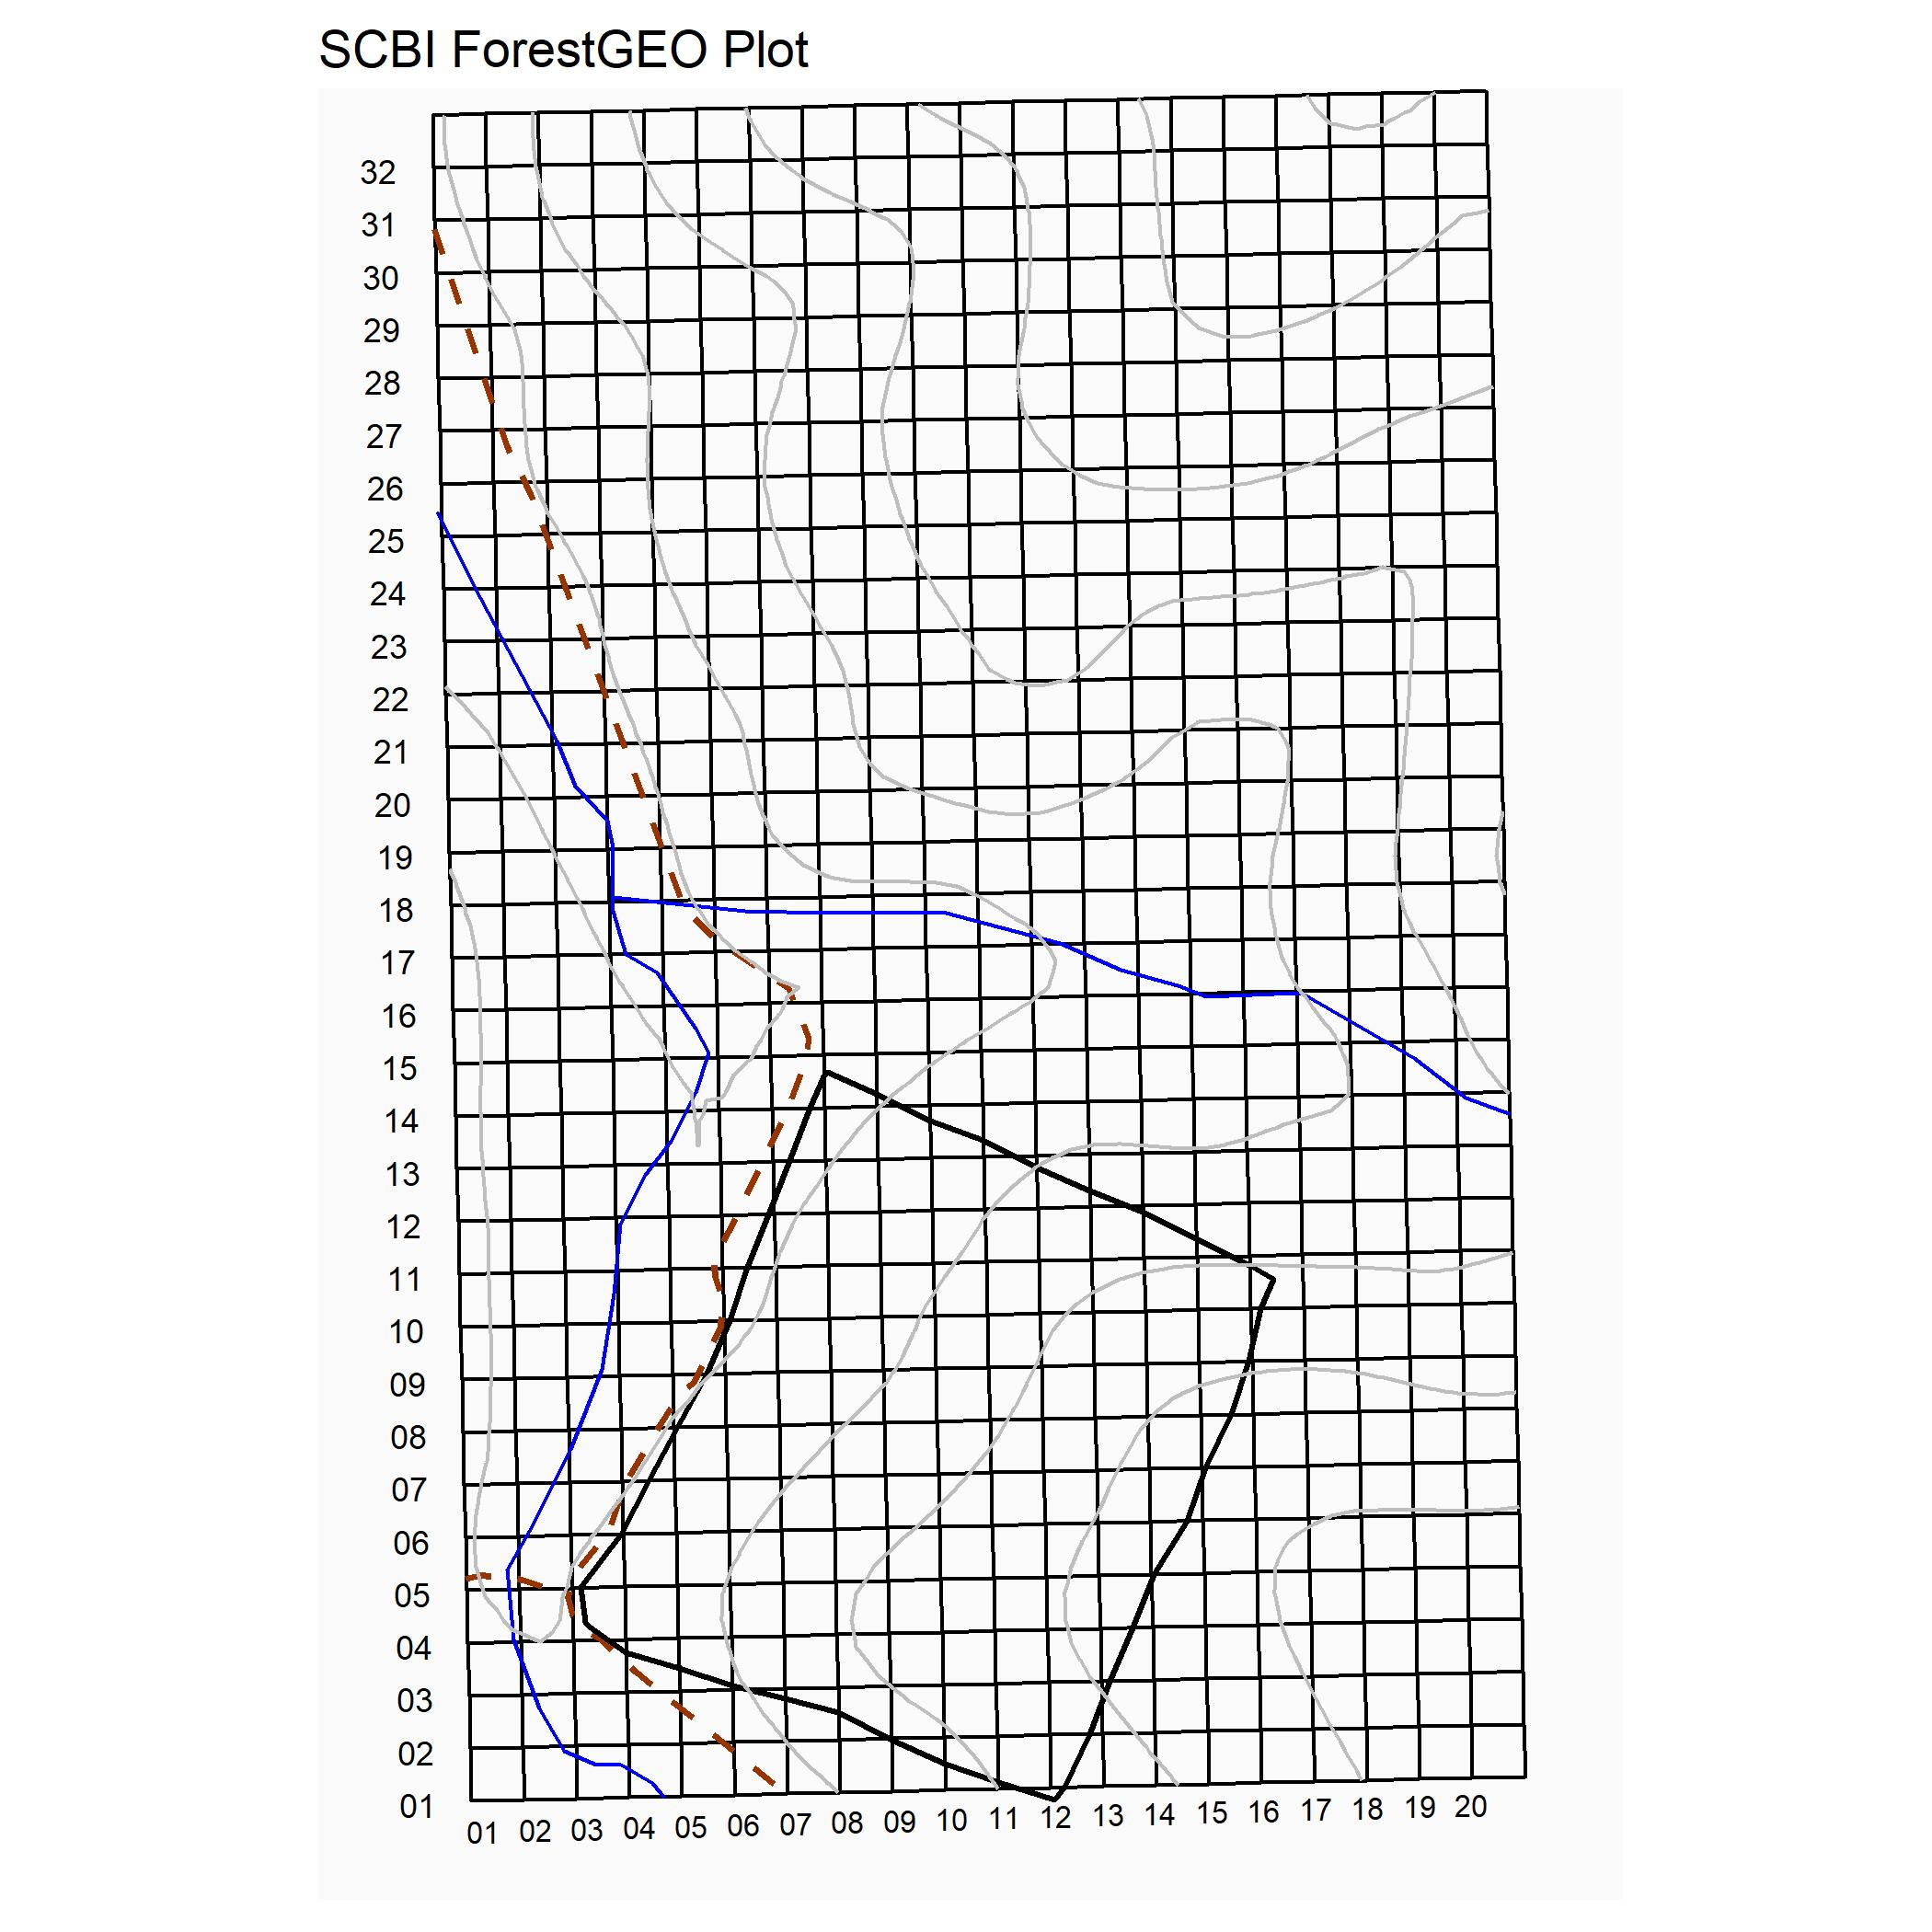
\includegraphics[width=1\linewidth]{tables_figures/ForestGEO_plot} \caption{Map of ForestGEO plot}\label{fig:Plot}
\end{figure}

\emph{how do we want to present Table S3? Would it be better as an image
of an excel file, since it's so large? Did we want to keep all
coefficients here?}

\begin{table}[!h]

\caption{\label{tab:Table S3}Top model variations for each drought scenario, with dAICc values <= 2}
\centering
\begin{tabular}{lrll}
\toprule
Modnames & Delta\_AICc & scenario & coef\\
\midrule
resist.value \textasciitilde{} height.ln.m+TWI.ln+PLA\_dry\_percent+mean\_TLP\_Mpa+(1|sp/tree) & 0.00 & trees\_all\_sub & NA\\
resist.value \textasciitilde{} position\_all+height.ln.m+TWI.ln+PLA\_dry\_percent+(1|sp/tree) & 0.34 & trees\_all\_sub & NA\\
resist.value \textasciitilde{} position\_all+height.ln.m+TWI.ln+PLA\_dry\_percent+mean\_TLP\_Mpa+(1|sp/tree) & 0.40 & trees\_all\_sub & NA\\
resist.value \textasciitilde{} height.ln.m+TWI.ln+rp+PLA\_dry\_percent+(1|sp/tree) & 0.52 & trees\_all\_sub & NA\\
resist.value \textasciitilde{} height.ln.m+TWI.ln+PLA\_dry\_percent+(1|sp/tree) & 0.57 & trees\_all\_sub & NA\\
\addlinespace
resist.value \textasciitilde{} position\_all+height.ln.m+TWI.ln+rp+PLA\_dry\_percent+(1|sp/tree) & 0.90 & trees\_all\_sub & NA\\
resist.value \textasciitilde{} height.ln.m+rp+PLA\_dry\_percent+mean\_TLP\_Mpa+(1|sp) & 0.00 & x1966 & NA\\
resist.value \textasciitilde{} height.ln.m+rp+PLA\_dry\_percent+(1|sp) & 0.54 & x1966 & NA\\
resist.value \textasciitilde{} position\_all+height.ln.m+rp+PLA\_dry\_percent+mean\_TLP\_Mpa+(1|sp) & 1.09 & x1966 & NA\\
resist.value \textasciitilde{} height.ln.m+PLA\_dry\_percent+(1|sp) & 1.43 & x1966 & NA\\
\addlinespace
resist.value \textasciitilde{} height.ln.m+TWI.ln+rp+PLA\_dry\_percent+mean\_TLP\_Mpa+(1|sp) & 1.98 & x1966 & NA\\
resist.value \textasciitilde{} position\_all+TWI.ln+rp+mean\_TLP\_Mpa+(1|sp) & 0.00 & x1977 & NA\\
resist.value \textasciitilde{} TWI.ln+rp+mean\_TLP\_Mpa+(1|sp) & 0.09 & x1977 & NA\\
resist.value \textasciitilde{} height.ln.m+TWI.ln+rp+mean\_TLP\_Mpa+(1|sp) & 1.12 & x1977 & NA\\
resist.value \textasciitilde{} position\_all+height.ln.m+TWI.ln+rp+mean\_TLP\_Mpa+(1|sp) & 1.91 & x1977 & NA\\
\addlinespace
resist.value \textasciitilde{} position\_all+height.ln.m+TWI.ln+rp+PLA\_dry\_percent+(1|sp) & 0.00 & x1999 & NA\\
resist.value \textasciitilde{} position\_all+height.ln.m+TWI.ln+rp+mean\_TLP\_Mpa+(1|sp) & 0.09 & x1999 & NA\\
resist.value \textasciitilde{} position\_all+height.ln.m+TWI.ln+rp+(1|sp) & 0.46 & x1999 & NA\\
resist.value \textasciitilde{} TWI.ln+rp+PLA\_dry\_percent+(1|sp) & 0.96 & x1999 & NA\\
resist.value \textasciitilde{} position\_all+height.ln.m+rp+mean\_TLP\_Mpa+(1|sp) & 1.03 & x1999 & NA\\
\addlinespace
resist.value \textasciitilde{} position\_all+height.ln.m+rp+PLA\_dry\_percent+(1|sp) & 1.19 & x1999 & NA\\
resist.value \textasciitilde{} TWI.ln+rp+mean\_TLP\_Mpa+(1|sp) & 1.33 & x1999 & NA\\
resist.value \textasciitilde{} position\_all+height.ln.m+TWI.ln+rp+PLA\_dry\_percent+mean\_TLP\_Mpa+(1|sp) & 1.85 & x1999 & NA\\
resist.value \textasciitilde{} position\_all+height.ln.m+rp+(1|sp) & 1.85 & x1999 & NA\\
\bottomrule
\end{tabular}
\end{table}

\begin{figure}
\centering
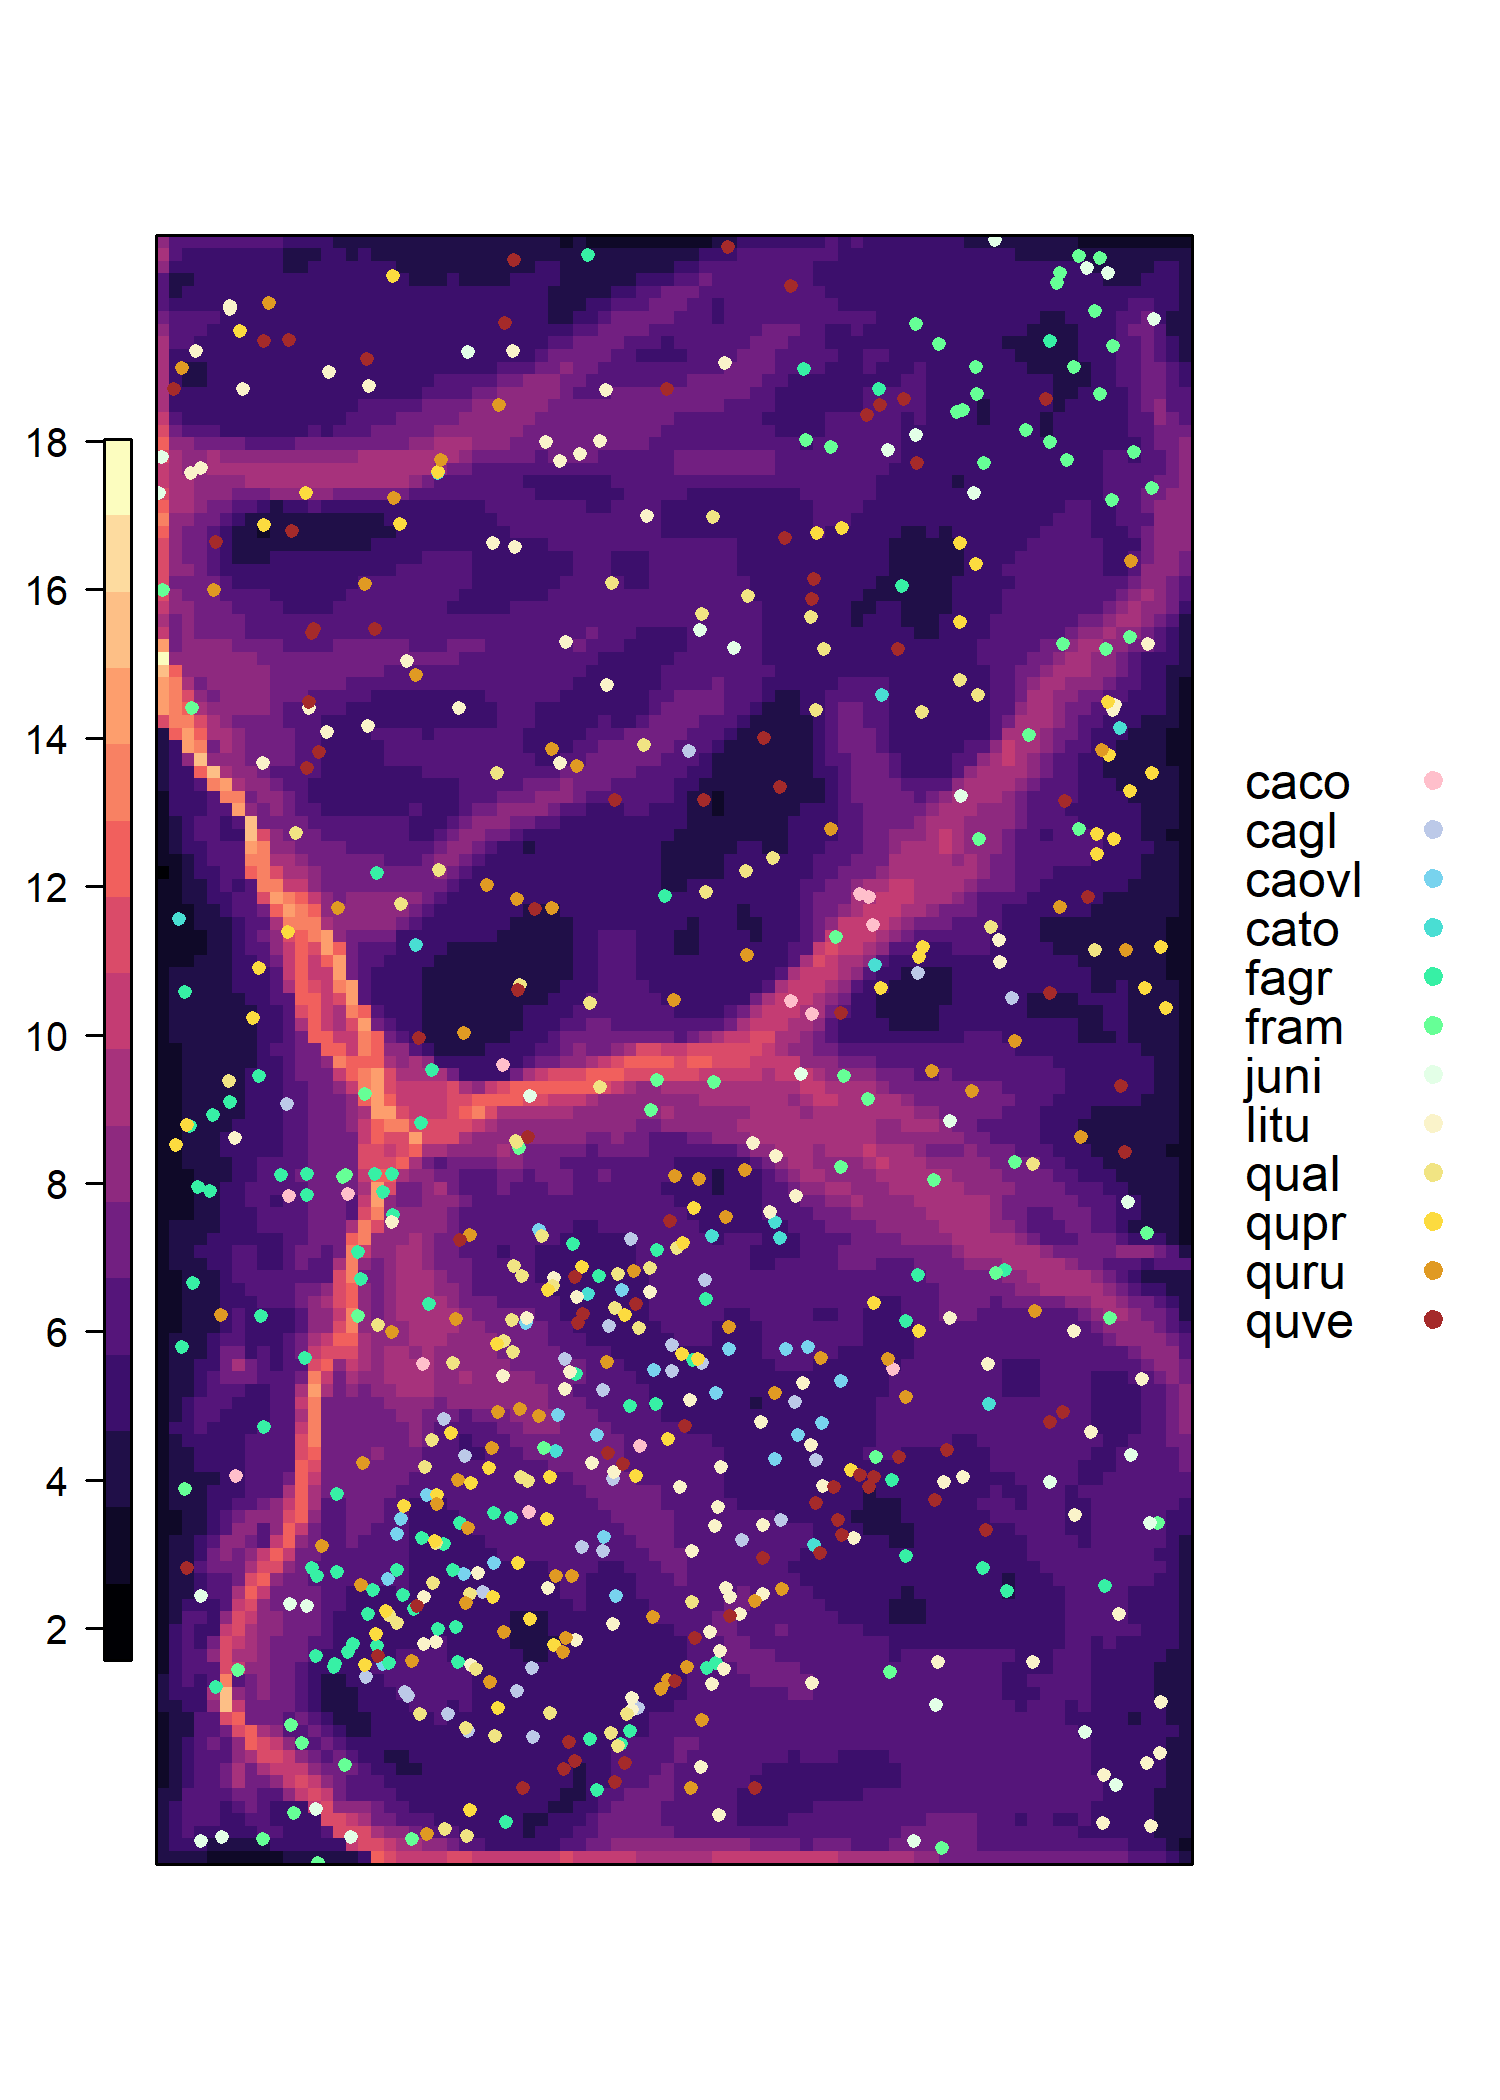
\includegraphics[width=5.20833in,height=\textheight]{tables_figures/FigureS3.png}
\caption{Location of cored trees}
\end{figure}

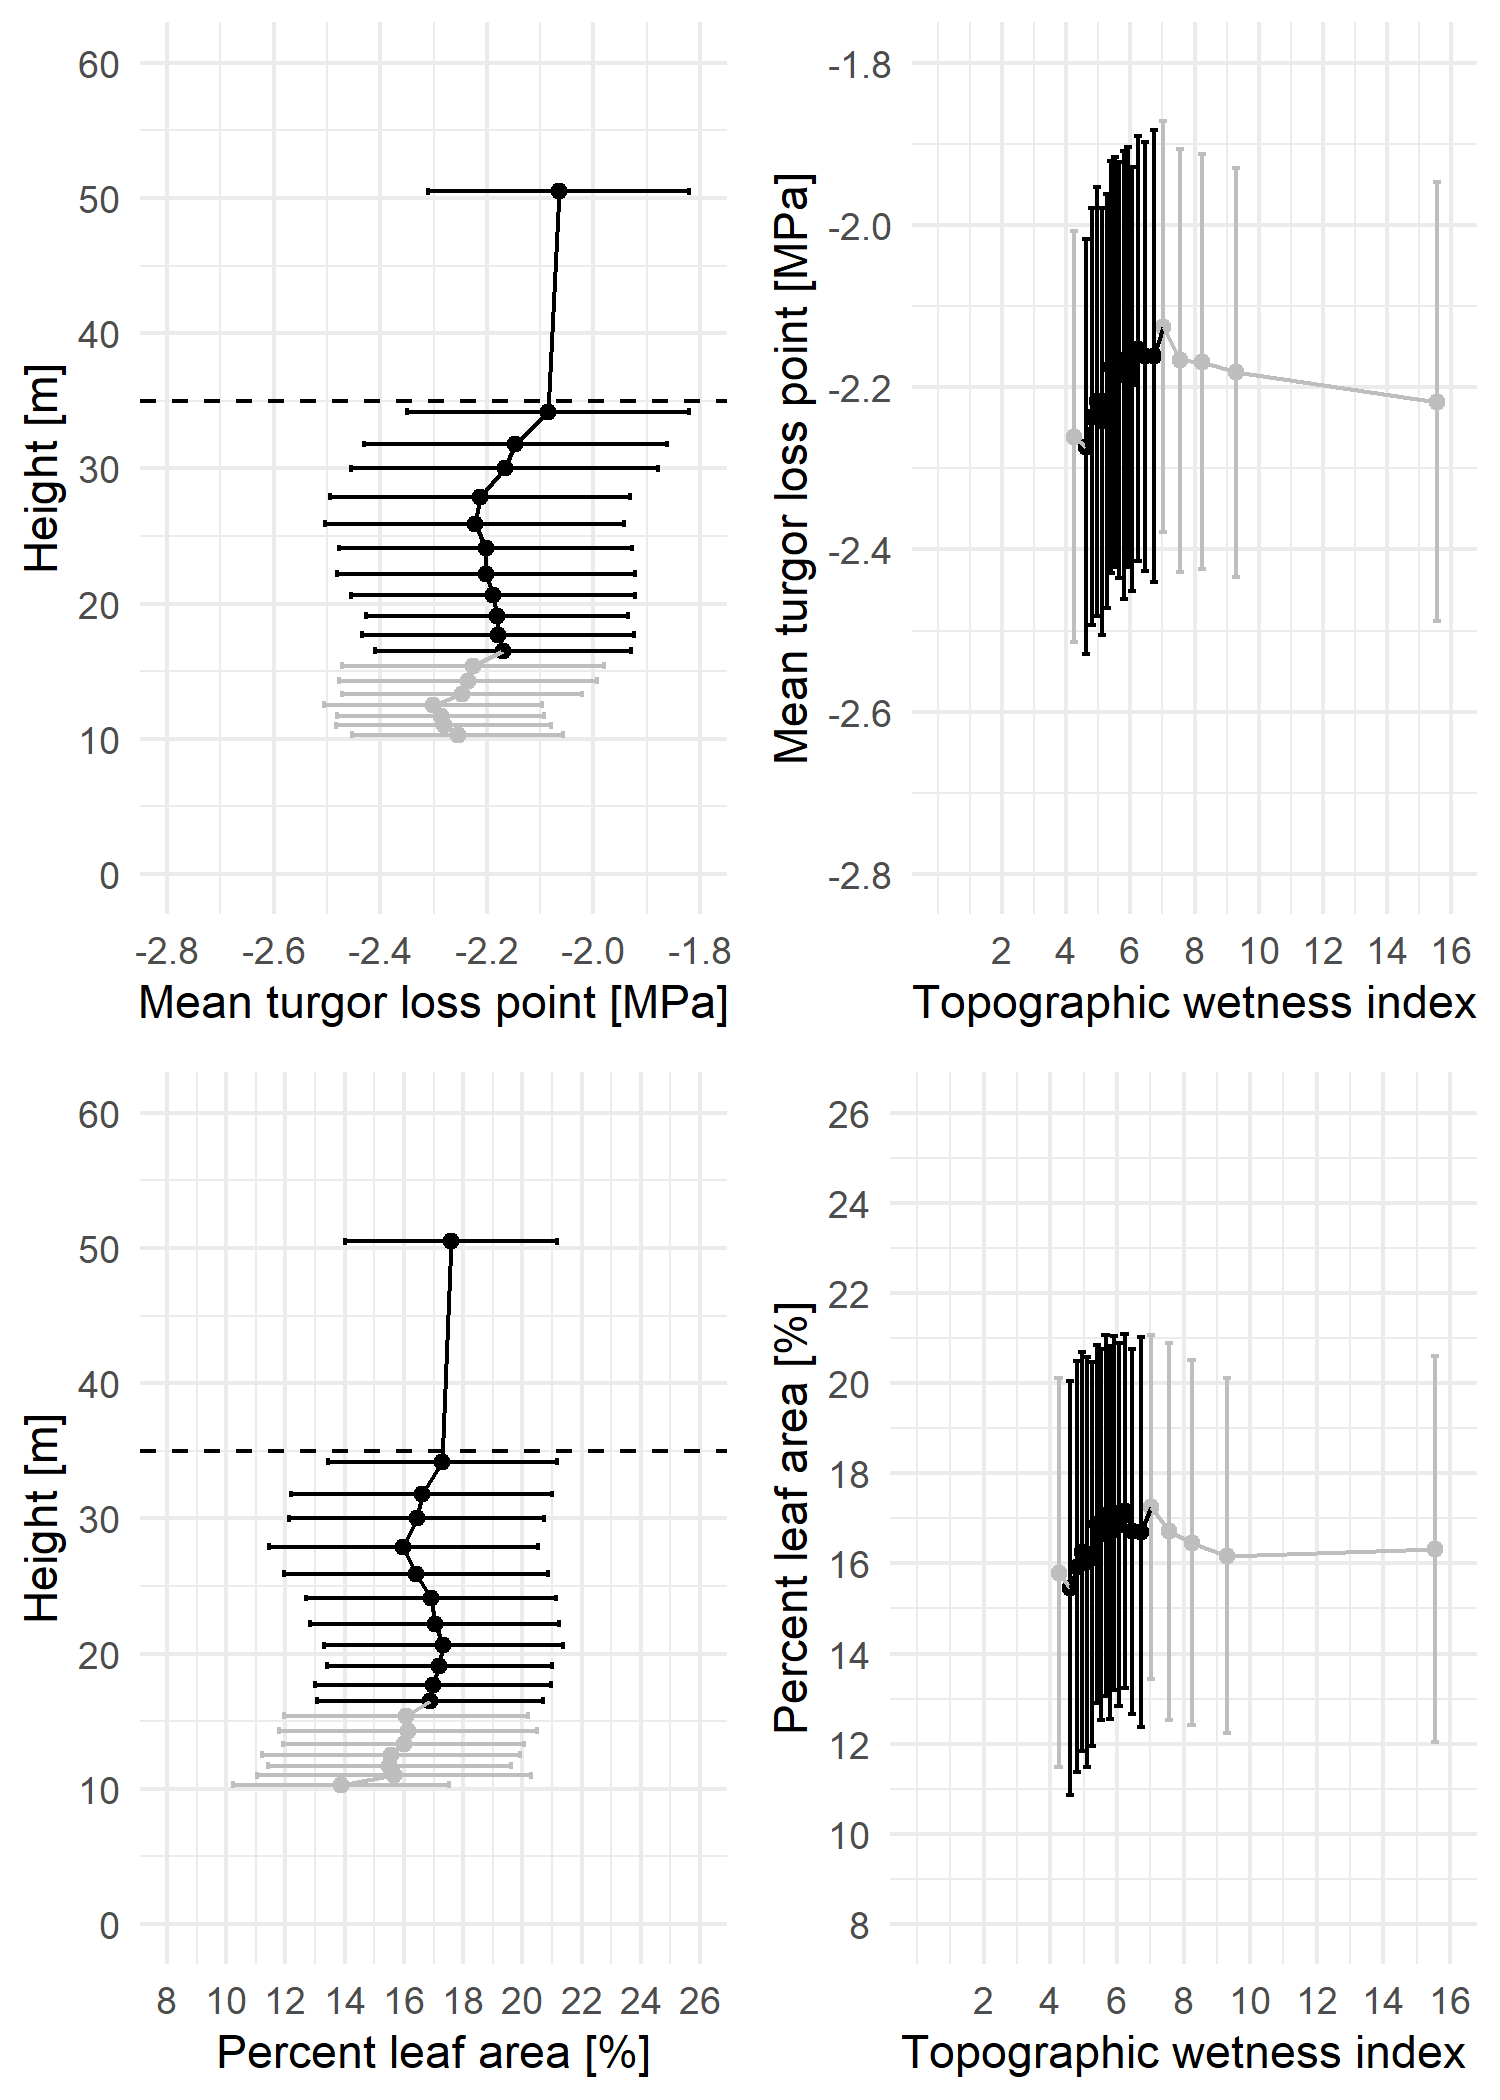
\includegraphics{tables_figures/FigureS1.png} (see Issue \#32)

\bibliography{book.bib,packages.bib}


\end{document}
